\chapter{Results} \label{chapResults}
\section{Photogrametry on Drone Forest Images}
An important first step in multiple approaches we used is understanding the structure of the forest scene. As one solution to this problem, we ran Agisoft Metashape with the parameters from Young et al. \cite{Young2022} on a variety of datasets. Three datasets shown in Figure \ref{fig:results:sfm} are representative of the types of data we experimented with. The first dataset, \textit{Stowe}, was collected with a lawnmower survey from a commodity drone. The locations of all the cameras were properly estimated and the results look good throughout. Some geometry of the trees can be seen, but much of the fine detail is lost, which is common for photogrammetry. The next dataset is \textit{Warton}, which was collected with the custom payload at an off-nadir angle of 60 degrees from horizontal and manual flight pattern observing roughly the same region from different angles. All of the cameras were properly aligned, but the quality of the mesh varies dramatically. In the center where there are multiple observations, the results are fairly good. However, both the structure and texture become blurrier farther away from the central area. This is likely because there are fewer camera views to triangulate and those regions are farther away. This mesh is darker than the \textit{Stowe} it was underexposed, due to a fixed exposure between collects. It is important to balance under- and over-exposure, especially in regions with different brightness. A further consideration is that longer exposures are more prone to motion blur, which is especially common while the drone is turning.
Finally, \textit{Coimbra} is a dataset where the drone follows a path between trees. The data is captured with the custom payload facing forward at 30 degrees from horizontal. A large portion of this trajectory appeared to be roughly accurate. However, in multiple instances, a set of cameras and the associated mesh were rotated relative to the correct orientation. This resulted in odd artifacts that made the mesh effectively unusable. Furthermore, the level of visual detail was fairly low.


\begin{figure}[H]
    \subfloat{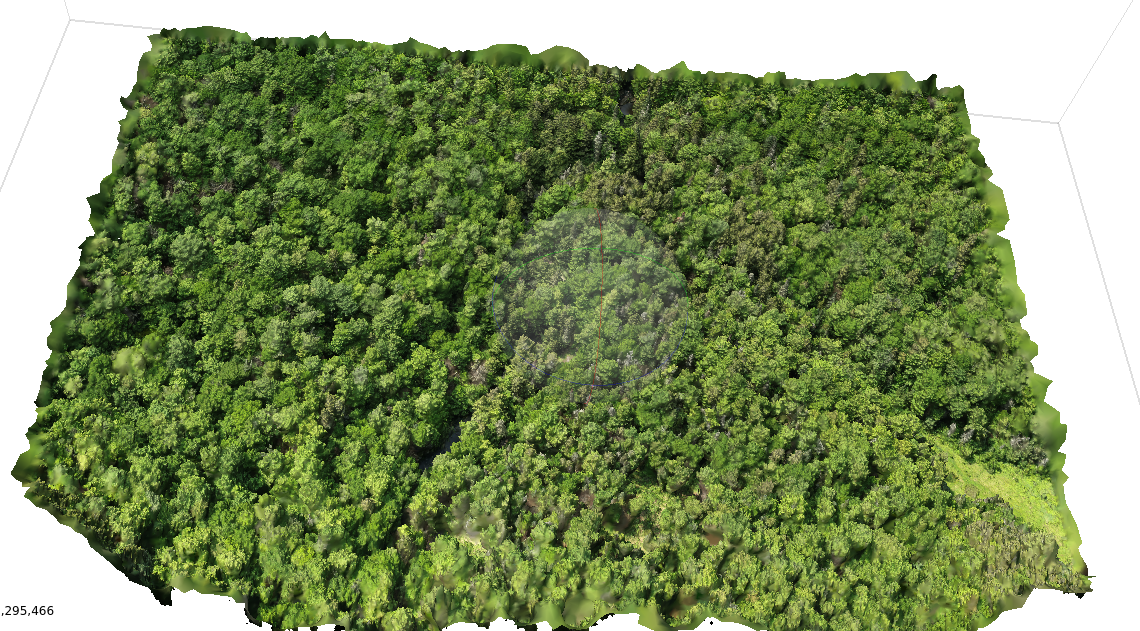
\includegraphics[width=0.45\textwidth]{figs/results/geometric_understanding/stowe_anew_collect_000_zoomed_out.png}}
    \hfill
    \subfloat{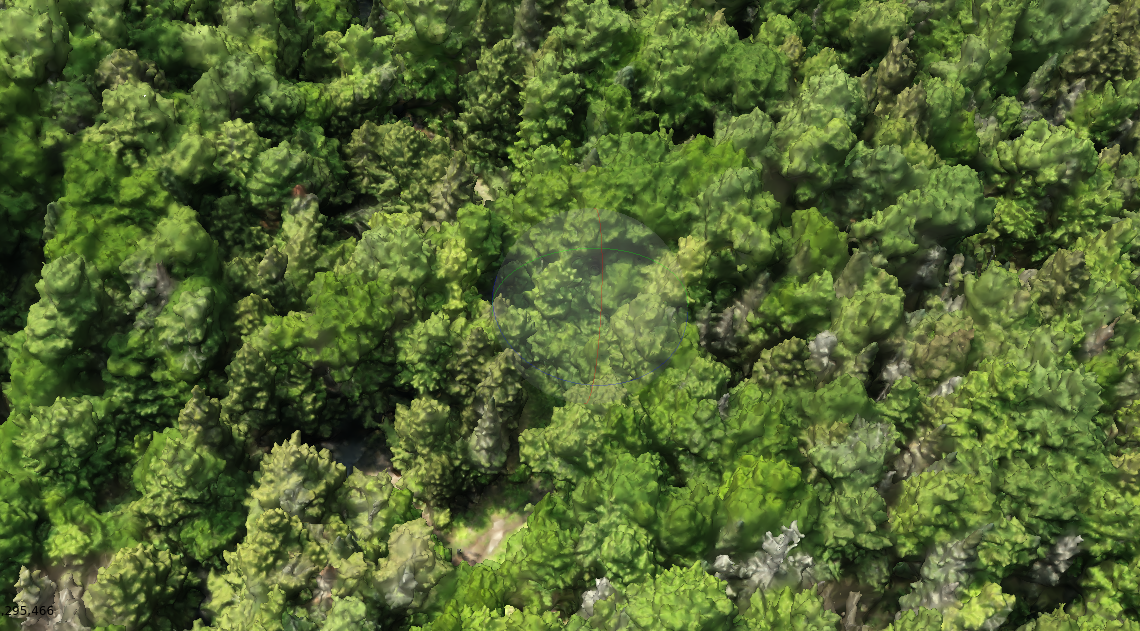
\includegraphics[width=0.45\textwidth]{figs/results/geometric_understanding/stow_anew_collect_000_zoomed_in.png}}\\
        
    \subfloat{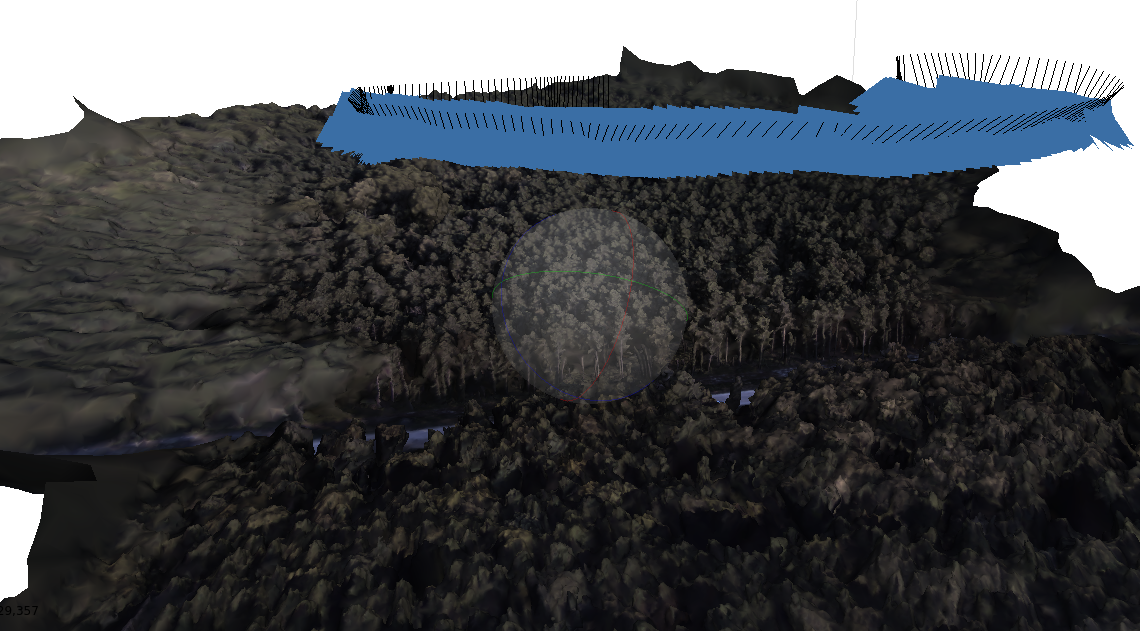
\includegraphics[width=0.45\textwidth]{figs/results/geometric_understanding/burn_zoomed_out.png}}
    \hfill
    \subfloat{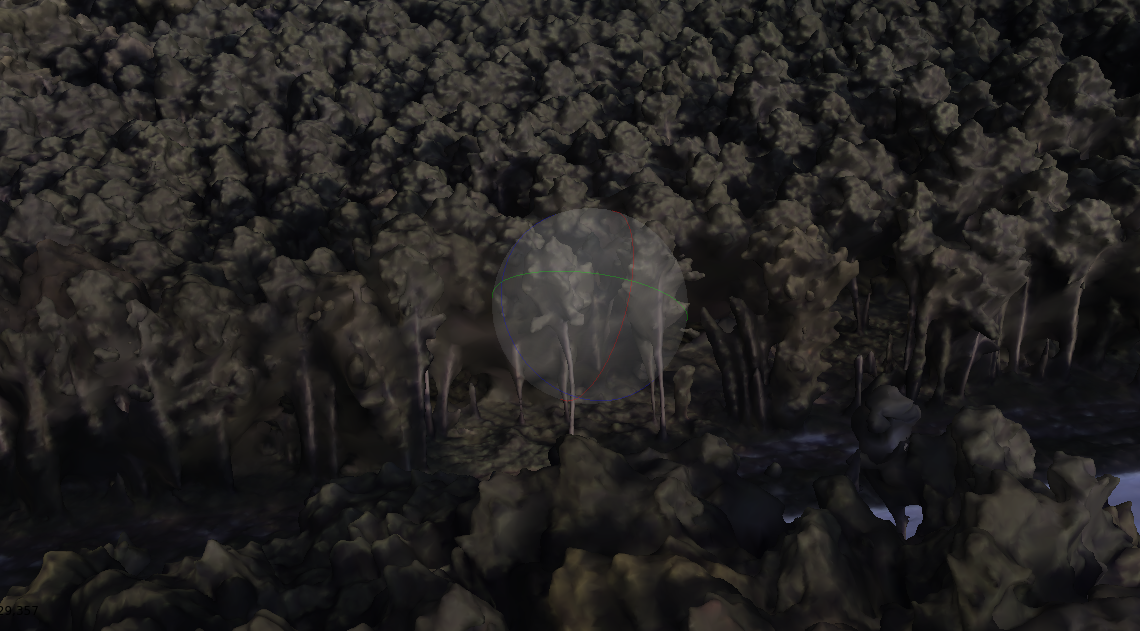
\includegraphics[width=0.45\textwidth]{figs/results/geometric_understanding/burn_zoomed_in.png}}\\
    
    \subfloat{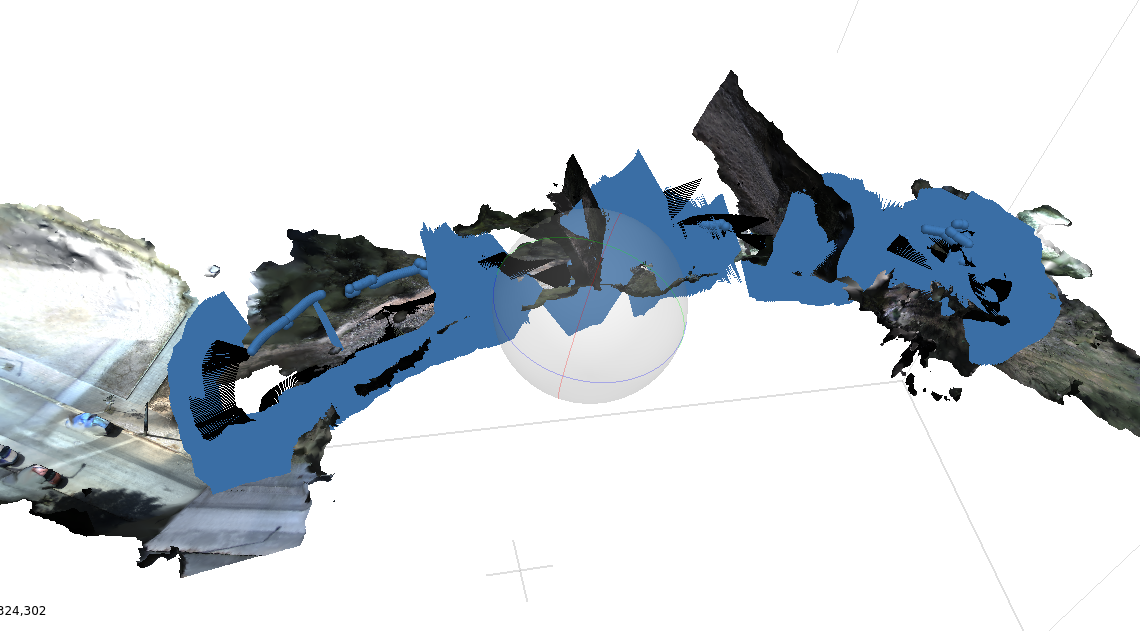
\includegraphics[width=0.45\textwidth]{figs/results/geometric_understanding/coimbra_zoomed_out.png}}
    \hfill
    \subfloat{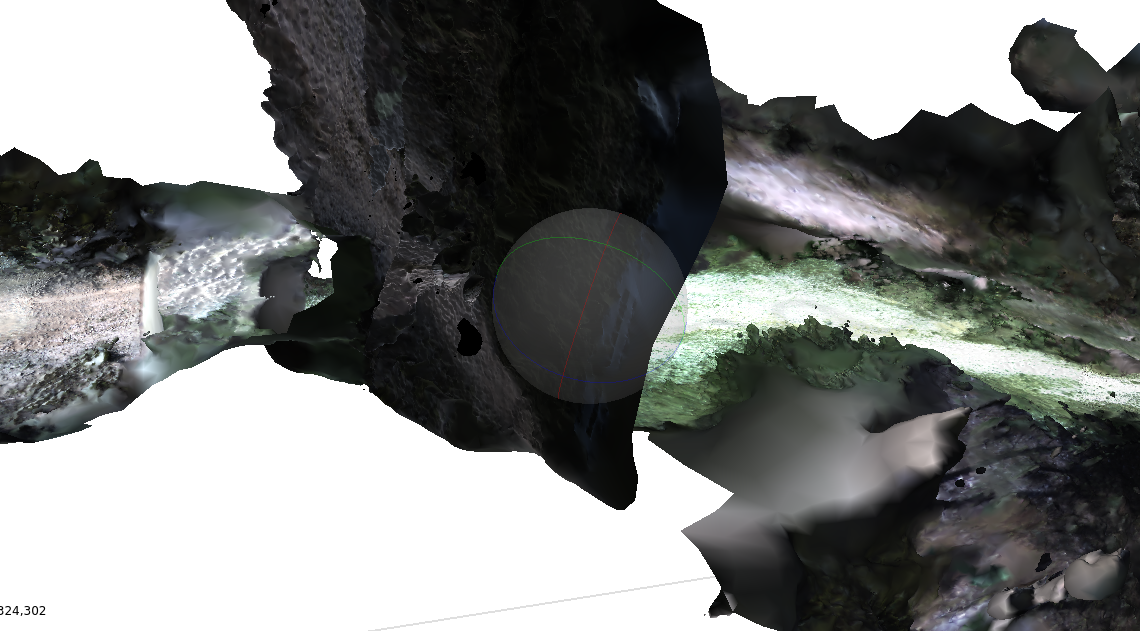
\includegraphics[width=0.45\textwidth]{figs/results/geometric_understanding/coimbra_zoomed_in.png}}
    \caption{3D reconstructions using Agisoft Metashape on three different environments. From top to bottom, they are a lawnmower pattern with a commodity drone,  The full map is shown to the left and a zoomed-in inset is shown to the right.}
    \label{fig:results:sfm}
\end{figure}

These results support the common practice of automated drone surveys using a lawnmower pattern since this method yielded consistently high-quality results across all the datasets we experimented on. However, it also shows that manual flight patterns over the canopy yield some useful data and challenging under-canopy conditions are somewhat successful. This suggests that traditional drone surveys are well-motivated, but further research on photogrammetry for more challenging forest scenarios may yield useful results.

%A practical consideration when working with these systems is the camera exposure. This is generally handled well by commodity systems, but may need to be hand-tuned on an experimental robotic system. If the exposure is too long, especially in the case of rapid drone movement, there can be motion blur which degrades the quality of reconstructions. Similarlly, both over and under-exposed images lead to fewer features to match between images and areas of minimial information in the final mesh.  

\section{Simultanous Localization and Mapping in Forest Environments}

\begin{figure}[H]
   \centering
   %----primera subfigura----
   \subfloat[]{
        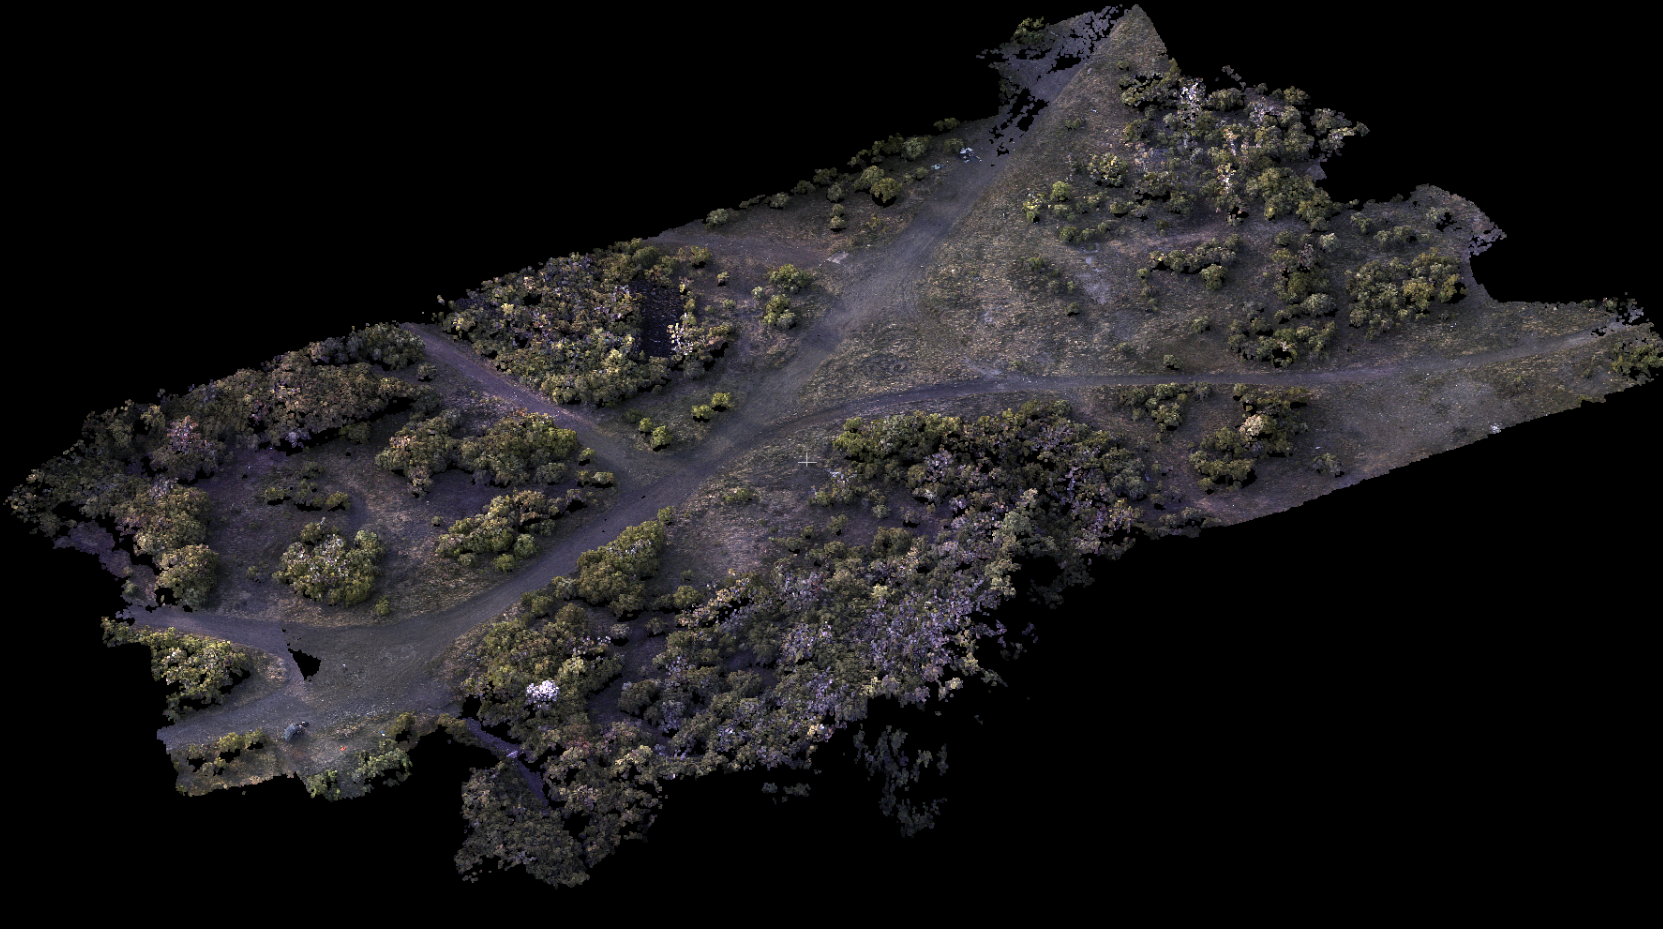
\includegraphics[width=0.465\textwidth]{figs/results/geometric_understanding/metashape_cloud_v3.png}}
   %\hspace{0.1\linewidth}
   \subfloat[]{
        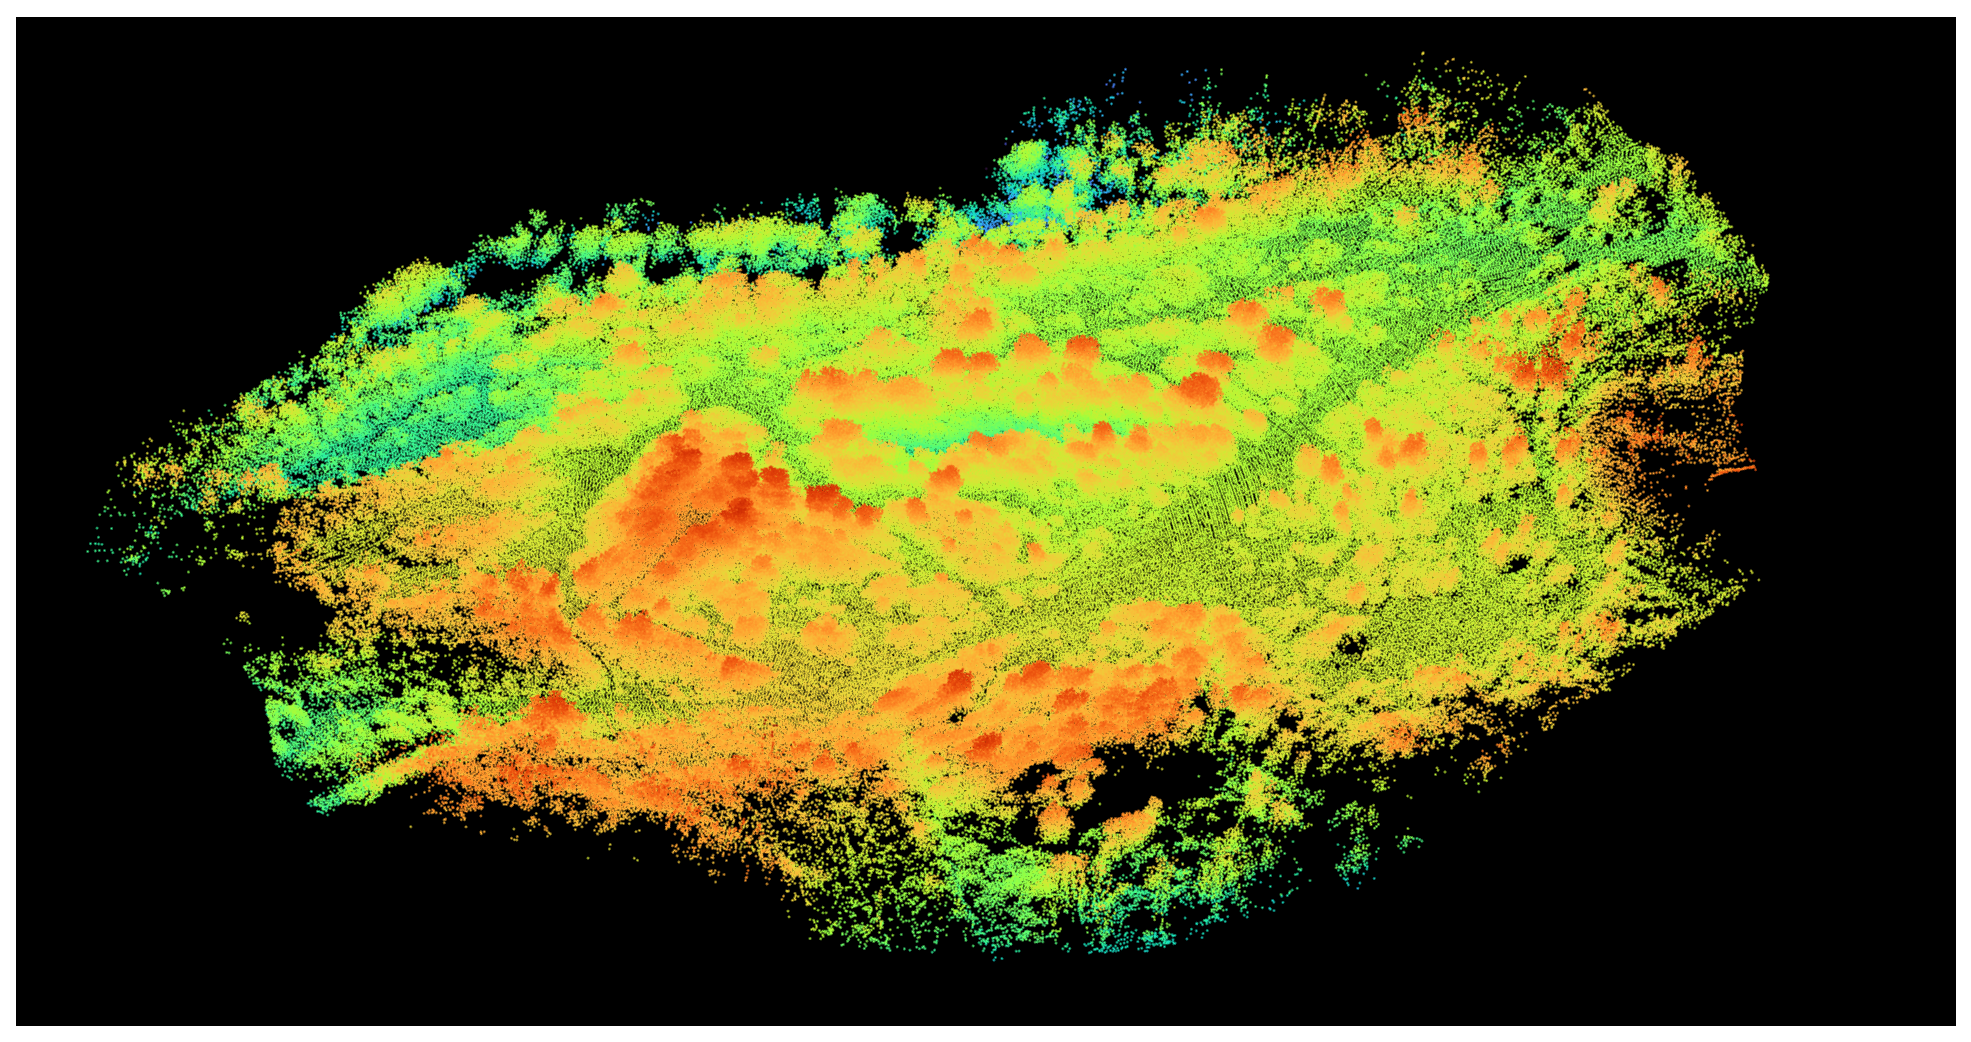
\includegraphics[width=0.5\textwidth]{figs/results/geometric_understanding/slam_ptCloud.eps}}\\%\\[20pt]   
   \subfloat[]{
        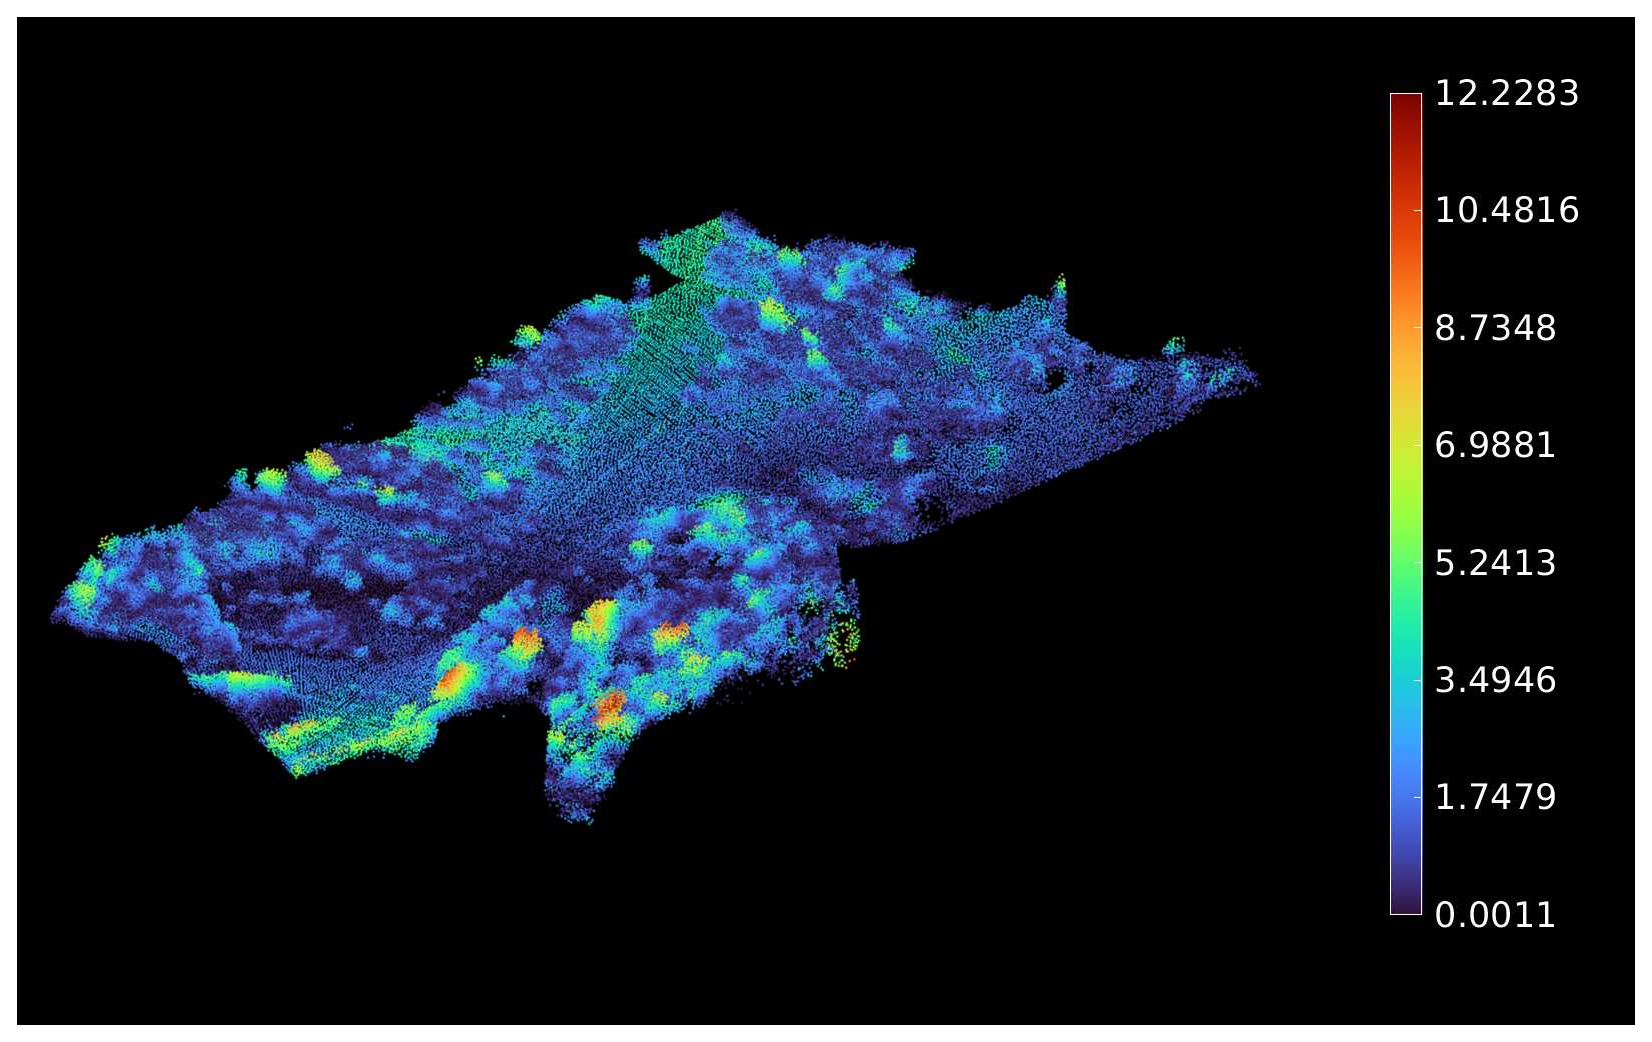
\includegraphics[width=0.5\textwidth]{figs/results/geometric_understanding/housedorff_distance.eps}}%\\[20pt]            
   \caption{Point cloud maps of the A) photogrammetry baseline, B) SLAM outcome. The two maps were compared using the Hausdorff distance, whose result is visualized as C) the SLAM map colored according to this metric. Note that the baseline and the SLAM clouds color maps correspond to RGB and height values, respectively. Analysis and figure provided by Francisco Yandun.}
   \label{fig:results:slam_photogrametry_comparison}
\end{figure}

We were interested in comparing the results of SLAM to photogrammetry because these two systems represent an interesting trade-off. SLAM approaches generally require multiple synchronized and calibrated sensors, with LiDAR being a common requirement. However, they can run in an online manner which can be used to inform robots' next actions. Photogrammetry requires only images, with optional GPS. The downside is it is computationally expensive and must be run in a batch after all the images have been collected.

We conduct this comparison on the \textit{Gascola} dataset that was surveyed with lawnmower coverage and the custom payload at a slight off-nadir angle. We ran photogrammetry using the default parameters. Francisco Yandun ran a tuned version of LIO-SAM \cite{Shan2020LIO-SAM:Mapping} and conducted a comparison between the two approaches.

As shown in Figure \ref{fig:results:slam_photogrametry_comparison}, the two maps agree fairly well in most regions. A notable source of high error is the tops of trees. In general, our qualitative assessment suggested that the SLAM approach was better at capturing these fine details compared to photogrammetry. This is because it had the benefit of explicit 3D data from LiDAR, while the photogrammetry approach had to infer 3D information from images. This often leads to sharp points and fine detail being lost. This shows that in offline applications of over-canopy mapping, photogrammetry is likely sufficient. 

\section{Tree Detection using Data at Multiple Scales}
We propose a set of experiments to explore different approaches to using multiple types of data. The baseline approach is applying the pre-trained DeepForest model to the aerial data. This requires no field measurements but is expected to produce low-quality detections because the model was trained on drone data at native resolution, which has significantly more texture. The next approach is using the pre-trained version of DeepForest on the drone data. This is expected to be significantly better than the aerial data because it is similar to what the model was trained on. The next two experiments involve fine-tuning the drone and aerial models on the small set of ground truth measurements. We expect that this fine-tuning will have a positive impact on the performance. Finally, we train a model for remote sensing data on the predictions from the drone. Even though these predictions are less accurate than manual labels, there are more of them, so this may improve performance.

In this experiment we generate predictions on two different modalities from the same \textit{Stowe} cite. The first is an orthomosaic derived from the drone and the second is NAIP imagery derived from aerial data. These predictions are shown in Figure \ref{fig:results:tree_det}. The predictions on drone data appear significantly better than those from the NAIP data. This is unsurprising because of the increased detail provided by the higher-resolution data. What is somewhat surprising is that fine-tuning the model did not appear to improve performance significantly. This suggests that the pretrained model already is already well-suited to this data, especially after appropriately matching the training resolution.

In Table \ref{tab:results:tree_det} we show the quantitative evaluation of the different approaches. We use precision, recall, and average intersection over union (IoU) to evaluate the results. The IoU represents the ratio of the overlap between a predicted and ground truth rectangle and the union of these two rectangles. A score of 0 means there is no overlap while a score of 1 means the prediction is perfect. The authors of DeepForest state that in ecological applications, an IoU of 0.4 is sufficient to be useful. Therefore, the precision metric represents the fraction of predicted trees that overlap with an IoU of at least 0.4 with a ground truth tree. The recall is the fraction of ground truth trees where a predicted tree overlaps with at least 0.4 IoU. Finally, the IoU column is the average IoU across all predictions with the best-matching ground truth tree.

\begin{table}[]
    \centering
    \begin{tabular}{|l|l|l|l|l|}
        \hline
        \textbf{Required data} & \textbf{Experiment} & \textbf{Recall} & \textbf{Precision} & \textbf{mIoU}\\
        \hline
        drone & Base ortho & 0.614 \pm 0.000 & 0.601 \pm 0.076 & 0.424 \pm 0.007\\ \hline 
        field + drone & Finetuned ortho & 0.608 \pm 0.012 & 0.617 \pm 0.070 & 0.432 \pm 0.009\\ \hline 
        NAIP & Base RS & 0.125 \pm 0.004 & 0.100 \pm 0.009 & 0.202 \pm 0.004\\ \hline 
        field + NAIP & Finetune RS & 0.282 \pm 0.004 & 0.221 \pm 0.032 & 0.271 \pm 0.017\\ \hline 
        drone + NAIP & Finetune RS on ortho base & 0.336 \pm 0.040 & 0.288 \pm 0.006 & 0.282 \pm 0.024\\ \hline 
        field + drone + NAIP & Finetune RS on ortho finetuned & 0.305 \pm 0.053 & 0.331 \pm 0.018 & 0.250 \pm 0.036\\ \hline 
\hline 
     \end{tabular}
    \caption{Tree detection results using multiple experimental strategies. The approaches are evaluated on precision and recall at an IoU threshold of 0.4 and the average IoU for all predictions.}
    \label{tab:results:tree_det}
\end{table}

These experiments present several key takeaways. As expected, drone data provides the best prediction results and is significantly better than remote sensing data. Fine-tuning the model on local data helped marginally in the case of drone data but more significantly in the case of NAIP data. This is understandable because the DeepForest model was pretrained on drone data from representative environments but not NAIP data. Finally, a model for NAIP data trained on drone predictions was better than a pre-trained model but worse than a model trained solely on a small set of annotations. This suggests that the errors in the drone predictions propagate into even larger errors in the remote sensing predictions. Overall, these approaches show that predictions from drone data are likely to be useful in a variety of ecological applications, but NAIP cannot be used for accurate tree detection using the current methods. However, it's possible that even these low-quality predictions could be used for some tasks such as estimating the number of trees or registering datasets by using trees as landmarks.

\begin{figure}[H]
    \subfloat{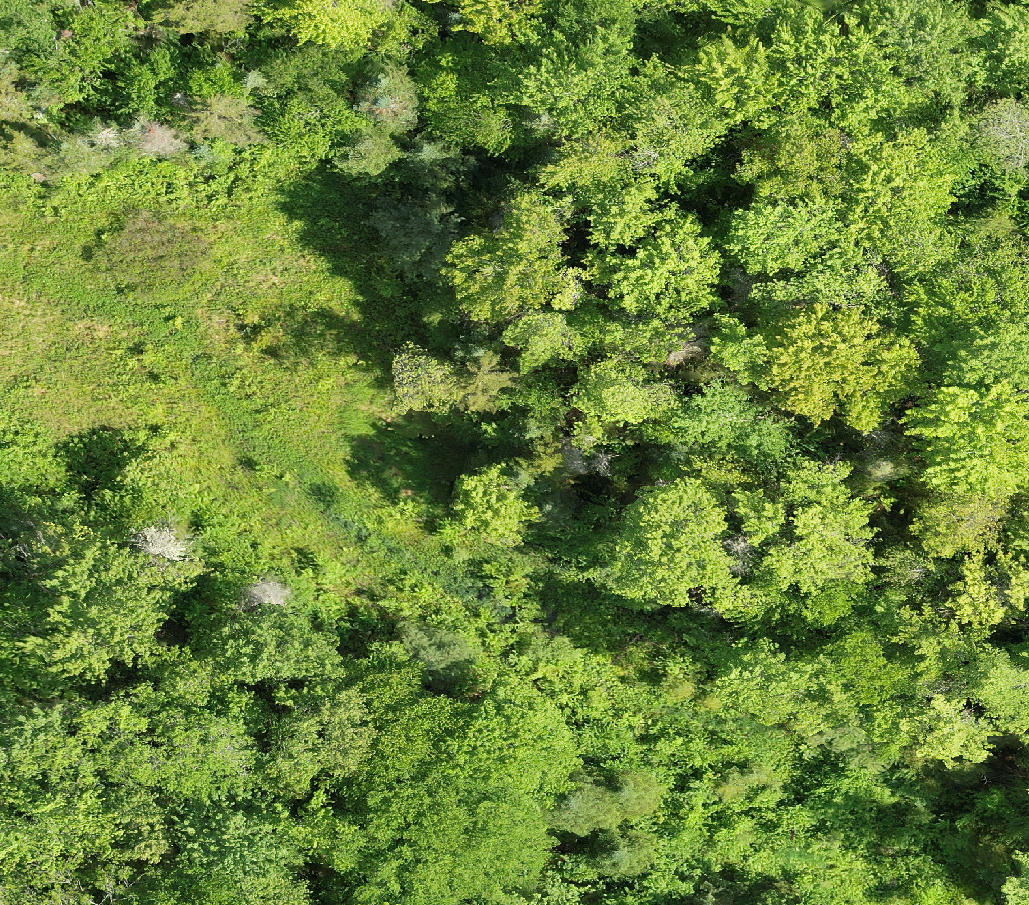
\includegraphics[width=0.40\textwidth]{figs/results/tree_detections/QGIS_VIS/base_image.png}}
    \hfill
    \subfloat{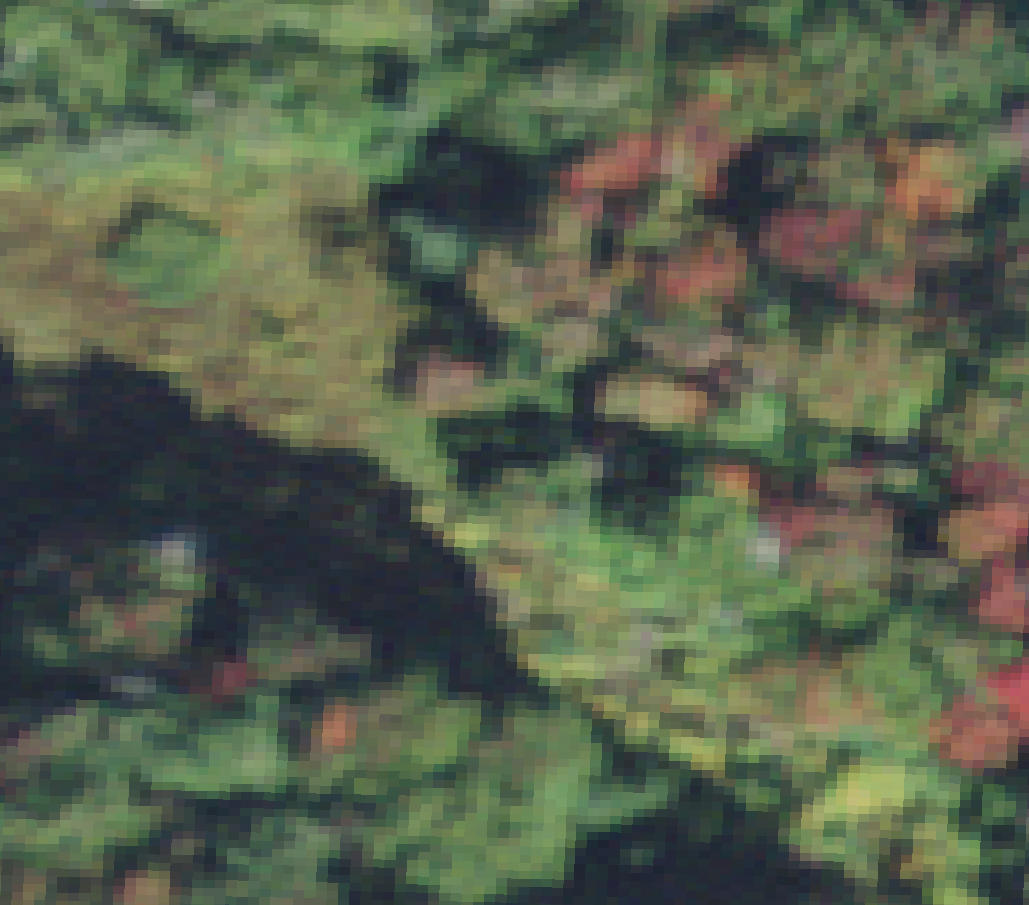
\includegraphics[width=0.40\textwidth]{figs/results/tree_detections/QGIS_VIS/naip_image.png}}
    \vfill
    \subfloat{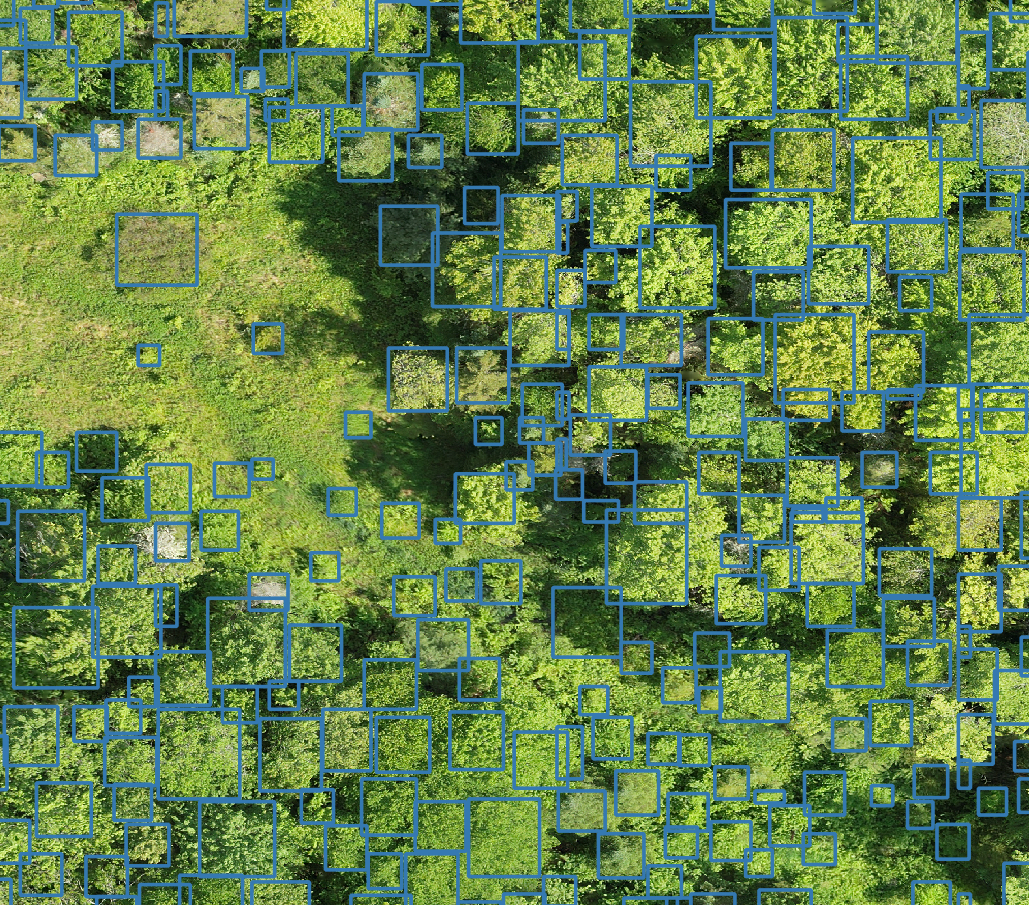
\includegraphics[width=0.40\textwidth]{figs/results/tree_detections/QGIS_VIS/drone_base.png}}
    \hfill
    \subfloat{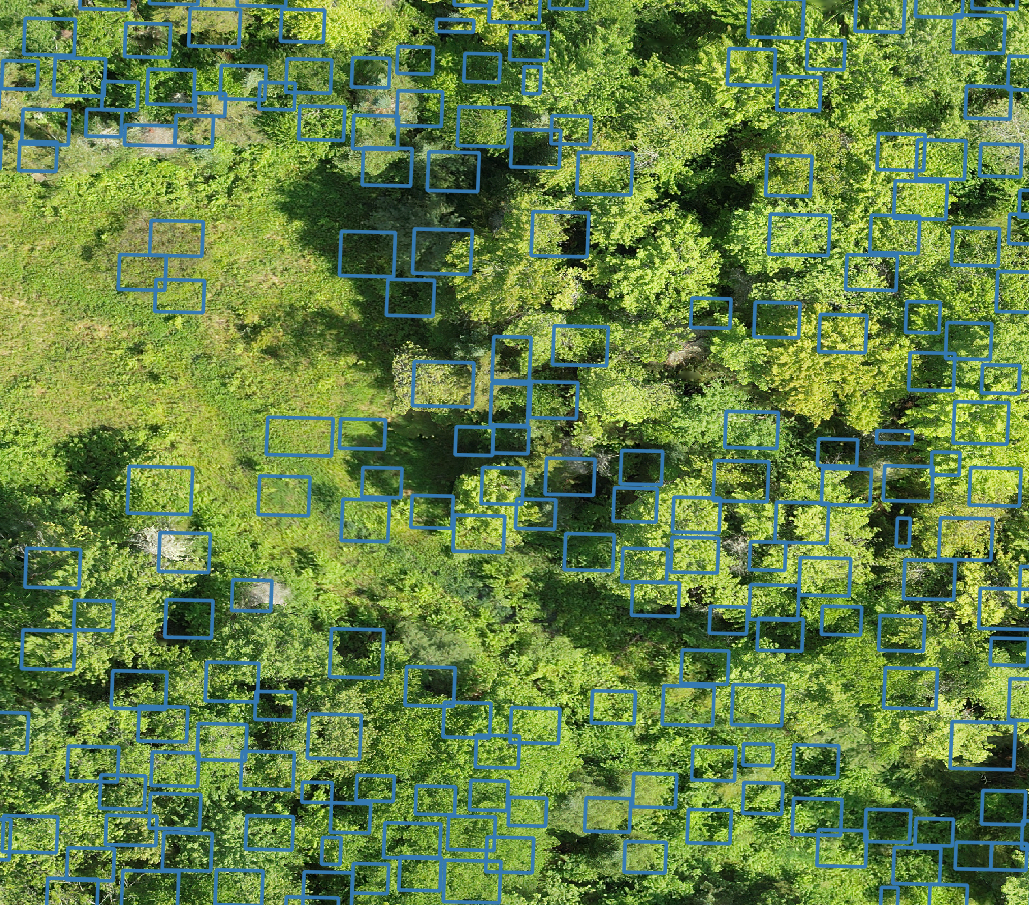
\includegraphics[width=0.40\textwidth]{figs/results/tree_detections/QGIS_VIS/naip_base.png}}
    \vfill
    \subfloat{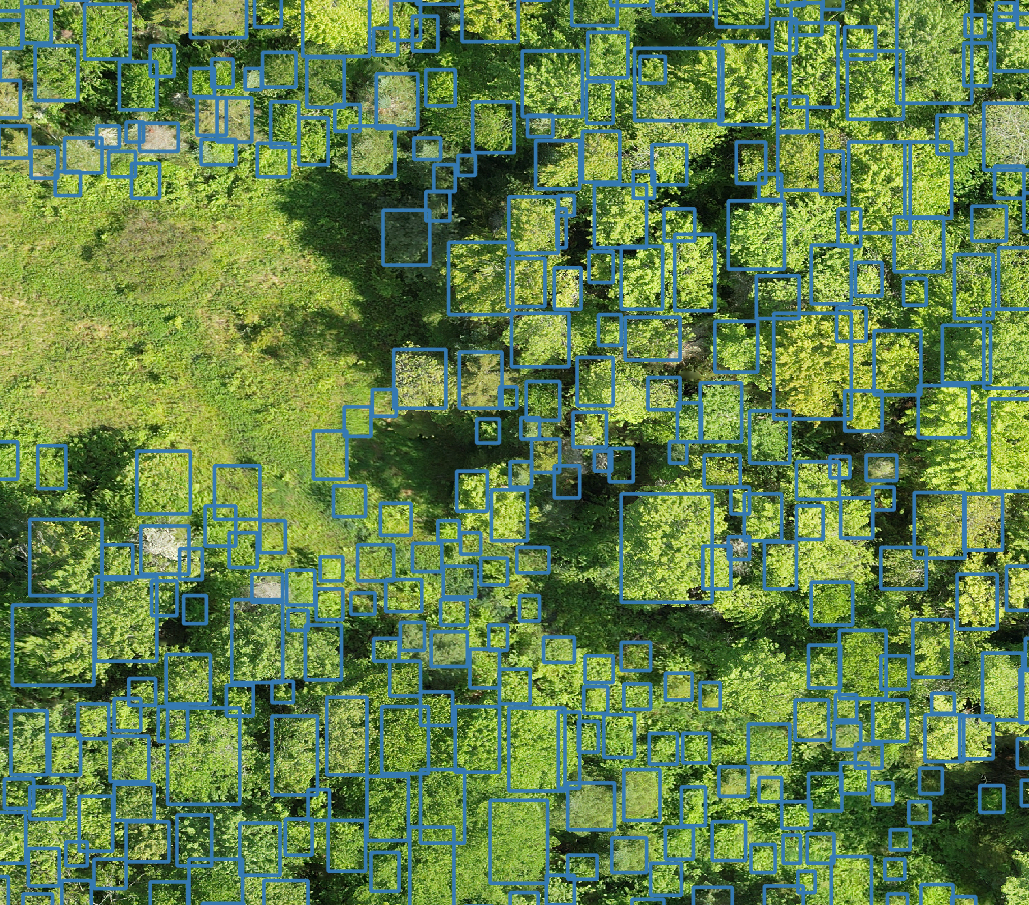
\includegraphics[width=0.40\textwidth]{figs/results/tree_detections/QGIS_VIS/drone_retrained.png}}
    \hfill
    \subfloat{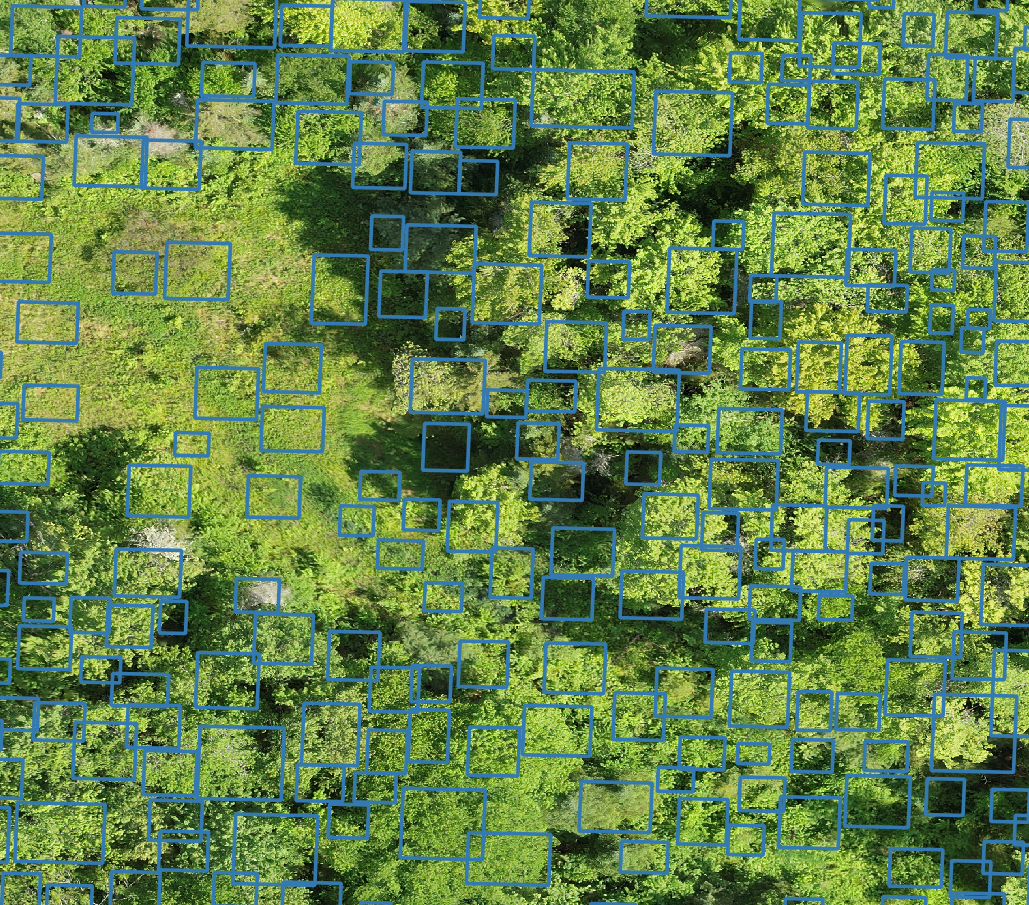
\includegraphics[width=0.40\textwidth]{figs/results/tree_detections/QGIS_VIS/naip_retrained.png}}
    \caption{Tree detections on a drone versus aerial data with and without fine-tuning on local data. Results for orthomosaics are on the left and NAIP is on the right. The first row is the input data, the second is the predictions from the base model, and the final is the predictions from the fine-tuned model. All predictions are visualized over drone data for clarity.
    }
    \label{fig:results:tree_det}
\end{figure}

\begin{figure}
    \centering
    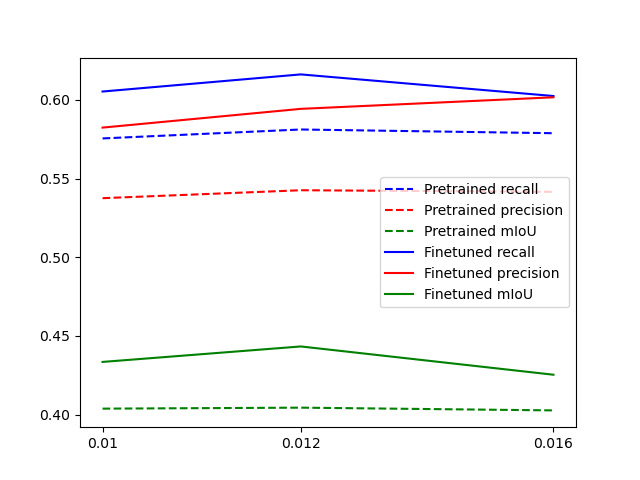
\includegraphics{figs/results/tree_detections/metrics.png}
    \caption{Tree detection metrics for drone data versus resolution}
    \label{fig:results:drone_resolution}
\end{figure}


\section{Semantic Mapping for Vegetation Classification}
The goal of this work is to build a 3D map of the environment that is annotated with the type of vegetation at each location. A challenge of this work is that we did not have access to field-reference data for the true locations of the different types of vegetation. Therefore, we conduct much of our quantitative evaluation on the semantic segmentation predictions, which can be more easily compared to human-labeled images. 

\subsection{Image Segmentation}
We conduct two experiments related to semantic segmentation. The first is a study using under-canopy data to determine the potential for synthetic pretraining and the impact of the number of training images on performance. The second is an evaluation of the model we used in over-canopy mapping with a small set of training examples.
\subsubsection{Sete Fonte Experiment}

\begin{figure}
   % First row
   \centering
    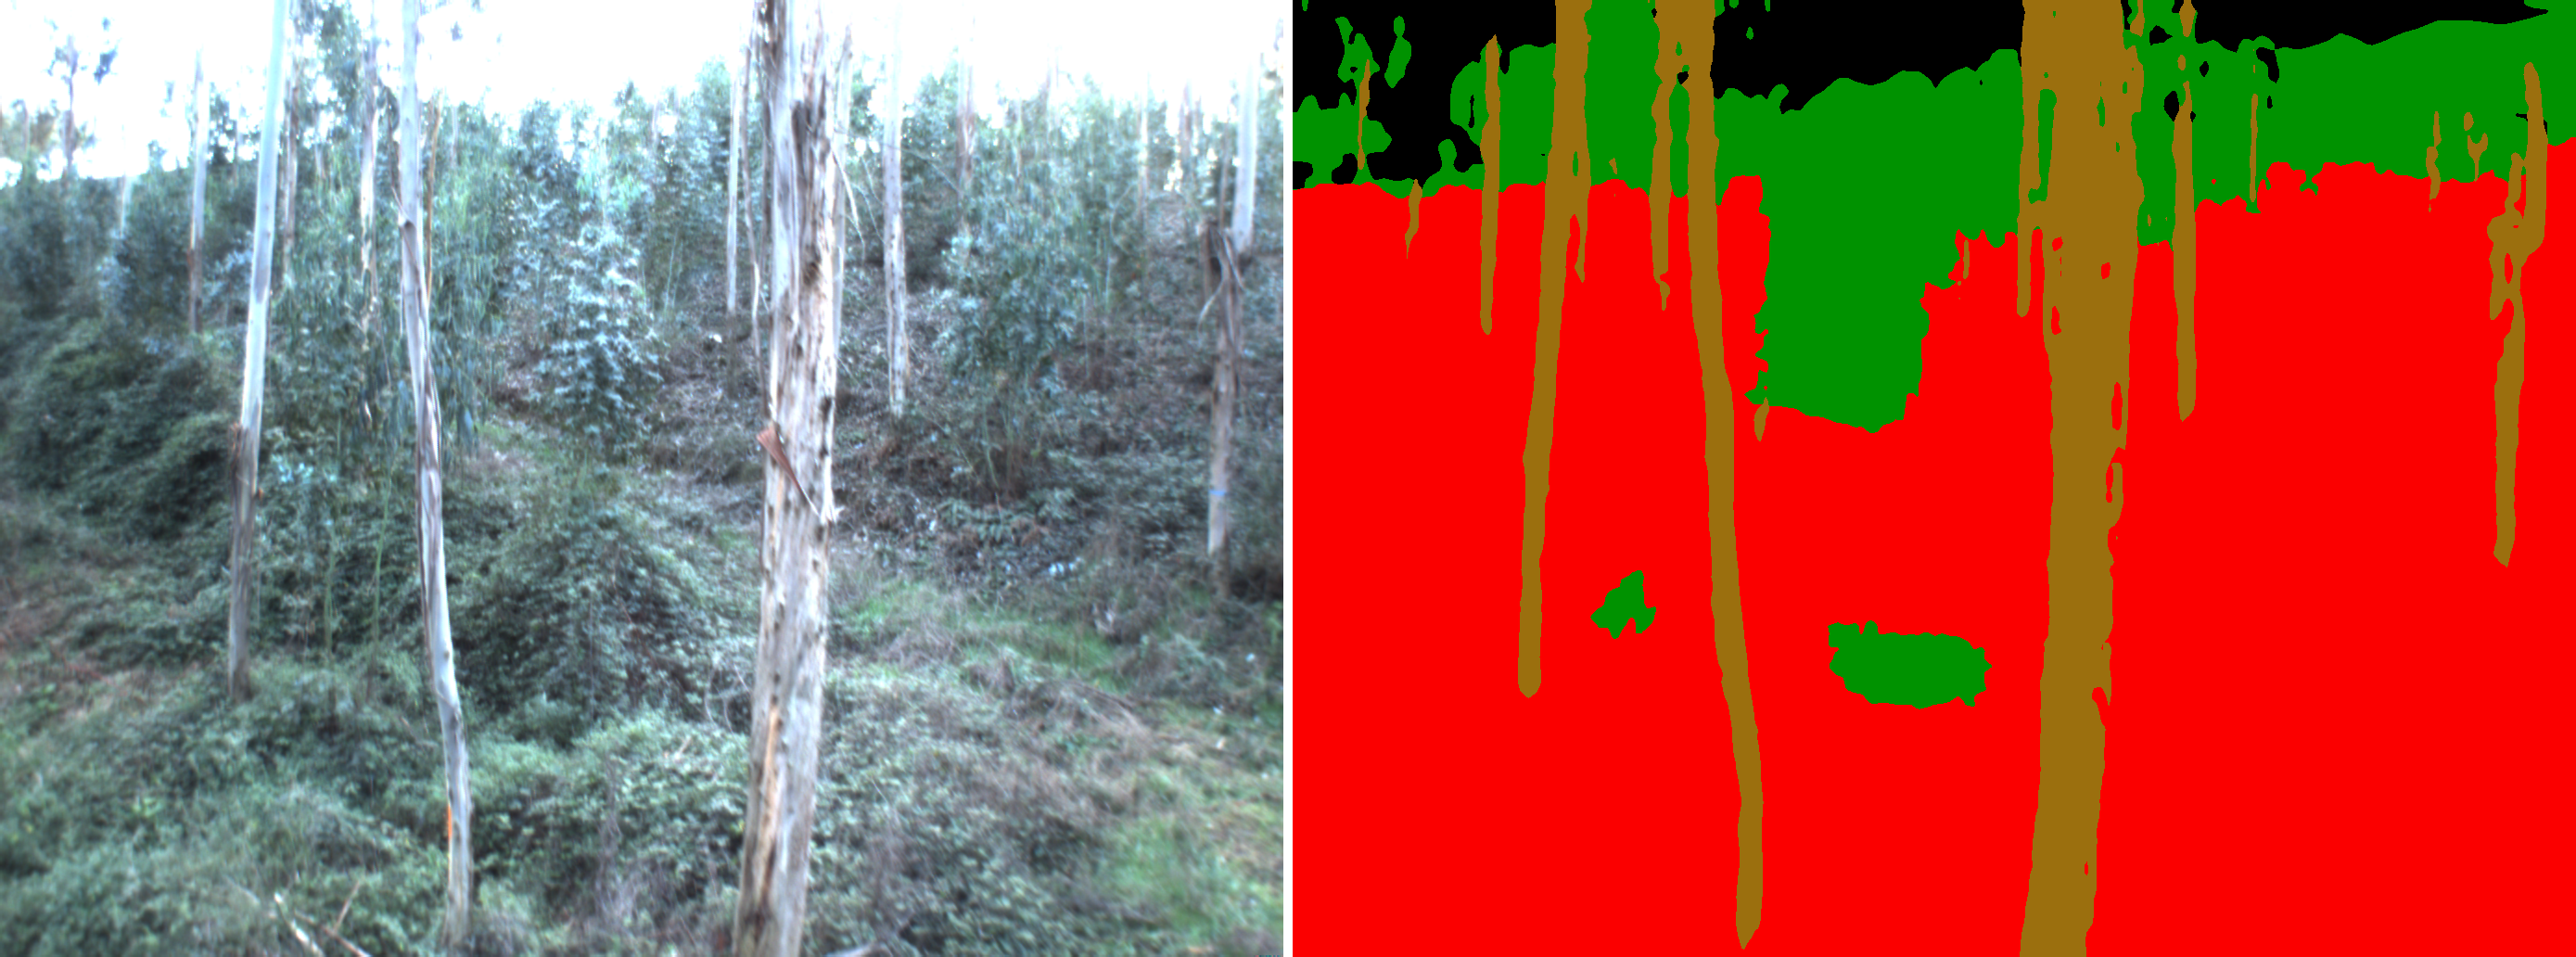
\includegraphics[width=\linewidth]{figs/results/semantic_segmentation/SeteFontes/qualatative_001400.png}  
    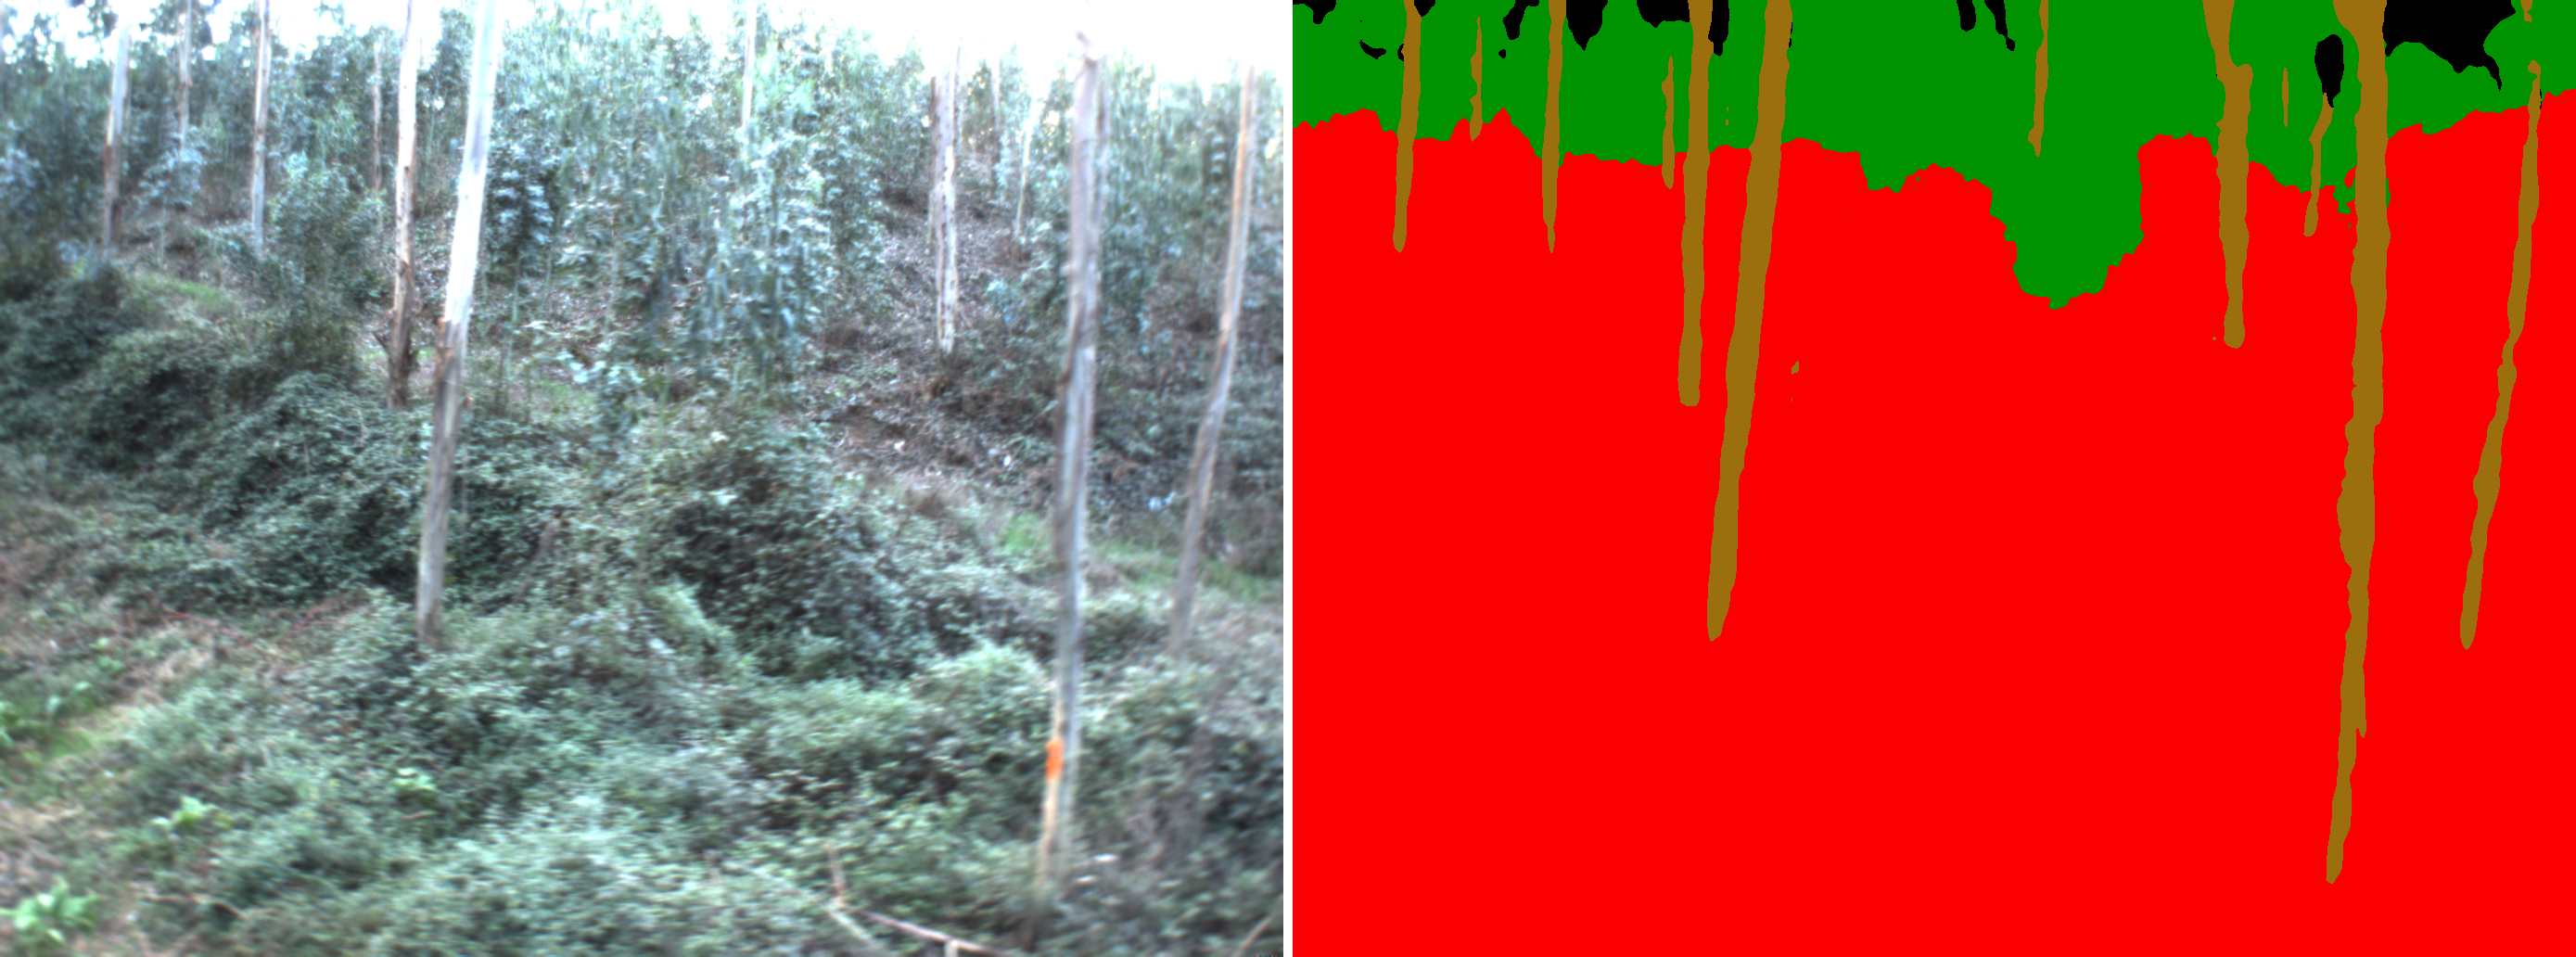
\includegraphics[width=\linewidth]{figs/results/semantic_segmentation/SeteFontes/qualatative_001600.png}  
    \caption{Predictions on the \textit{Oporto} dataset. Black is background, red is fuel, brown is trunks, and green is canopy.
    %Note that low trees are often predicted as fuel.
    } 
    \label{fig:results:oporto_semantic_seg_qual}
\end{figure}

Given the limited availability of real data and the labor-intensive nature of labeling to obtain ground truth, we explored the utility of models trained with simulated (\textit{synthetic}) data. We conducted three types of experiments: models trained solely with \textit{synthetic} data, models trained with real data (\textit{Setes Fontes}), and a mixture of both. For the last two cases, we trained different models with a variable number of real images to evaluate the performance of the model as the number of real labeled images varied. Thus, we conducted training experiments using (or adding) 7, 15, 21, 30, 60, 91, and 121 data points from the \textit{Setes Fontes} dataset. We trained for 10000 iterations and evaluated each model on 30 \textit{Setes Fontes} images not seen in the largest training split. We replicate this experiment over five folds of the data. For all three models the base networks were first pretrained with the \textit{CityScapes} dataset \cite{Cordts2016}. The mean Intersection over Union on the test set of each of these configurations is shown in Figure \ref{fig:results:semantic-size-pretraining}.

\begin{figure}[H]
    \centering
    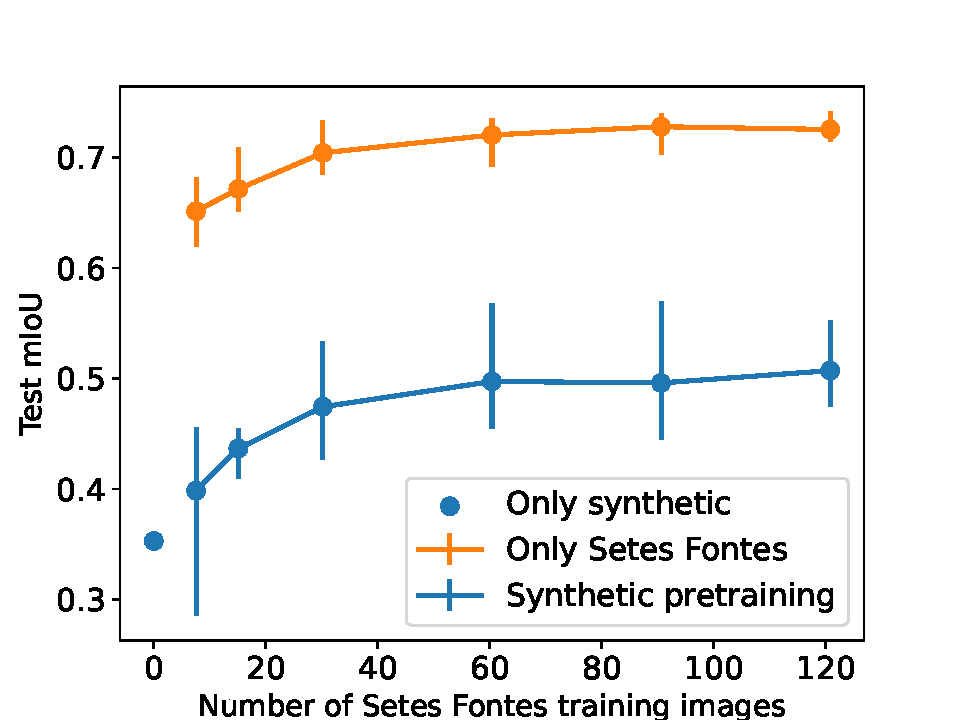
\includegraphics[width=0.7\textwidth]{figs/results/semantic_segmentation/synthetic_experiments_mious.pdf}
    \caption{Test mIoU for very few training images on the \textit{Setes Fontes} dataset.
    Error bars represent minimum and maximum results across the five folds of \textit{Setes Fontes}.}
    \label{fig:results:semantic-size-pretraining}
\end{figure}
It is interesting to note the relatively high performance of a model that used only 7 real images. Also, the model trained solely on synthetic data fails to generalize to real data, even after properly accounting for differences in mean and variance of both datasets. We found that combined real and synthetic data performs worse than training the same model only using real data. This suggests that the synthetic data comes from a completely different distribution than the real one, making its contribution detrimental. In the future, we plan to keep researching the causes of this interesting outcome. It is possible that simple attributes such as saturation or spatial resolution is the cause of this domain shift. Alternatively, it's possible that significantly more effort needs to be put into realistic simulations for them to be useful to train prediction models.
\begin{figure}[H]
    \centering
    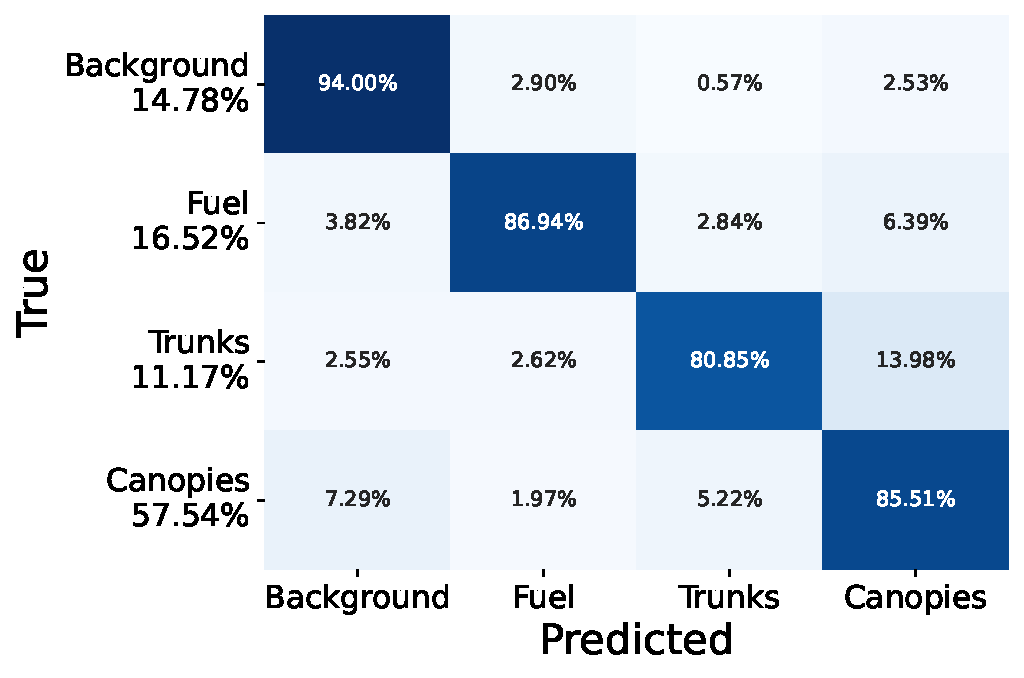
\includegraphics[width=0.6\columnwidth]{figs/results/semantic_segmentation/confusion_matrix.pdf} 
    \caption{Confusion matrix for the \textit{Setes Fontes} test datasets normalized per class with the true fraction of each class reported on the y axis labels.
    %Fuel is predicted fairly well, though it is fairly often confused for canopy, which is understandable given the visual similarity and the large fraction of canopy pixels.
    }
    \label{fig:results:sete_fontes_confusion_matrix}
\end{figure}

Since the model trained in 121 images ($80\%$ of the \textit{Setes Fontes} dataset) showed the best performance in these experiments, we conducted further experiments on it. The confusion matrix on the \textit{Sete Fontes} test set is shown in Figure \ref{fig:results:sete_fontes_confusion_matrix}. This shows that all four classes are predicted with reasonable accuracy. A common source of confusion is between trunks and canopies, which is understandable because they frequently overlap. Canopies are also confused for background, which includes the sky. Even though these two classes look very different, the sky can often be seen through the canopy, and the network miss-classifies these fine details. In most cases, this error is harmless because no LiDAR information should correspond to the sky pixels. Finally, the most common error for fuel is canopies, which is understandable because they are both leafy vegetation. Information about the height, either provided to the model or used in post-processing, could help disambiguate this confusion. 

Since we are mainly interested in the fuel instances, we aggregated the background, trunks, and canopies in a single non-fuel class. In that case, we obtained an IoU of 78.2\% and 95.3\% for \texttt{Fuel} and \texttt{Not Fuel}, respectively, which yields a mIoU of 86.7\%. This shows that our system performs well at its primary task of identifying fuel.

The end goal of this model is to be useful on the semantic mapping task on the \textit{Oporto} dataset, which wasn't seen during training. We show two qualitative examples of predictions in Figure \ref{fig:results:oporto_semantic_seg_qual}. The predictions still appear fairly accurate, despite the change in camera perspective from ground to aerial and different image characteristics. 


\subsubsection{Gascola Experiment}
In this experiment, we used two different datasets from \textit{Gascola} which partially covered the same region. We train on one dataset and test the model on the other. Because of the small number of images that we used in this experiment, these two datasets had different class distributions as shown in Figure \ref{fig:results:semantic_class_fracs}, though they had the same three main classes. Each of these three classes corresponded to a different aggregate class (Background, Canopy, and Fuel), so it was important to effectively tell them apart. 

\begin{figure*}[h!]
   \centering
   %----primera subfigura----
   \subfloat[]{
        \label{fig:train_class_frac}         %% Etiqueta para la primera subfigura
        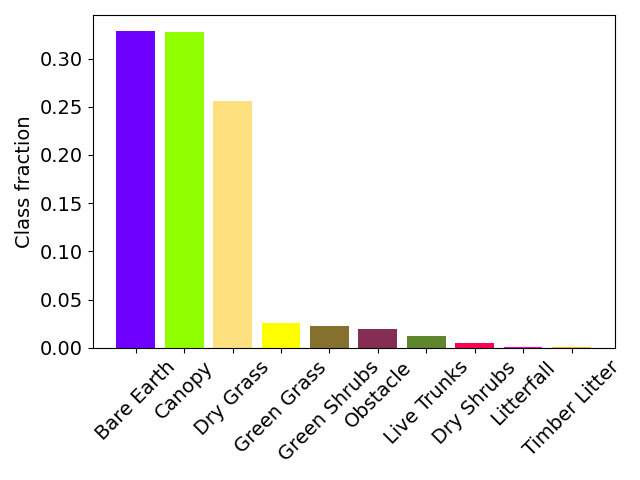
\includegraphics[width=0.5\textwidth]{figs/results/semantic_segmentation/class_fraction_train.png}}
   %\hspace{0.1\linewidth}
   \subfloat[]{
        \label{fig:test_class_frac}         %% Etiqueta para la segunda subfigura
        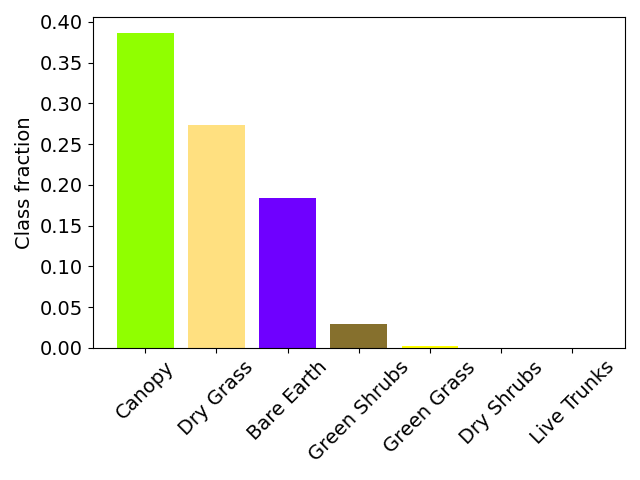
\includegraphics[width=0.5\textwidth]{figs/results/semantic_segmentation/class_fraction_test.png}}%\\[20pt]            
   \caption{This shows the fraction of pixels per class for A) the train set and B) the test set. Note that the three dominant classes Canopy, Bare Earth, and Dry Grass are common across both collections but the comparative frequencies are somewhat different. These correspond to our aggregate Canopy, Background, and Fuel classes respectively. The fractions of other classes are fairly small, and some from the training set are entirely absent in the test set.}
   \label{fig:results:semantic_class_fracs}                %% Etiqueta para la figura entera
\end{figure*}

The quality of predictions is shown in Table \ref{tab:results:semantic_eval}.  We summarized the IoU, precision, and recall for each class. The performance is fairly good on the most common classes, but, as expected drops on the rarer classes. As seen by the qualitative examples in Figure \ref{fig:results:semantic_gascola_qualitative}, there are instances where the predictions on the granular classes are incorrect, but the aggregate class is correct.

\begin{table}[ht!]
    \centering
\begin{tabular}{ccccc}
% \hline
\toprule
\textbf{Class} & \textbf{IoU} & \textbf{Precision} & \textbf{Recall} \\ \midrule
% \hline
Canopy & 70.05 & 84.77 & 80.13 \\
Dry Grass & 79.7 & 93.75 & 84.17 \\
Bare Earth & 78.53 & 88.12 & 87.83 \\
Green Shrubs & 3.27 & 21.72 & 3.71 \\
Green Grass & 0.0 & 0.0 & 0.0 \\
Dry Shrubs & 0.0 & 0.0 & 0.0 \\
Live Trunks & 0.05 & 0.05 & 84.09 \\
\bottomrule
% \hline
\end{tabular}
\caption{Evaluation results of the SegNext \cite{Guo2022SegNeXt:Segmentation} network with the Anderson Fuel Model \cite{anderson1981aids} for semantic segmentation in a forestry environment.}
\label{tab:results:semantic_eval}
\end{table}


\begin{figure*}[h!]
   \centering
   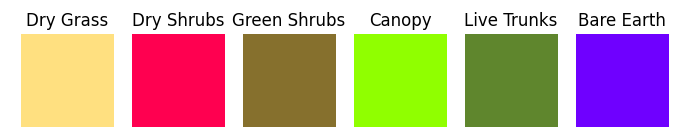
\includegraphics[width=0.63\textwidth]{figs/results/semantic_segmentation/Gascola/safeforest_all_classes_flat.png}
   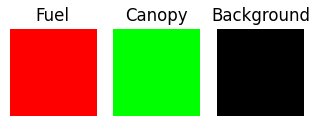
\includegraphics[width=0.33\textwidth]{figs/results/semantic_segmentation/Gascola/safeforest_classmap_compressed_flat.png}
   \includegraphics[width=\textwidth]{figs/results/semantic_segmentation/Gascola/000000_rgb_img.png}
   \vspace{0pt}
   \includegraphics[width=\textwidth]{figs/results/semantic_segmentation/Gascola/000005_rgb_img.png}
   \vspace{0pt}
   \includegraphics[width=\textwidth]{figs/results/semantic_segmentation/Gascola/000010_rgb_img.png}
   \vspace{0pt}
   \includegraphics[width=\textwidth]{figs/results/semantic_segmentation/Gascola/000015_rgb_img.png}
   \vspace{0pt}
   \caption{
   Qualitative semantic mapping results from the test set. The results are shown both for the predicted classes and the aggregated ones, with colors visualized in the top rows.
   White regions in the ground truth represent areas that were ambiguous to the human annotator. Overall the predictions match the ground truth well and boundaries are well-defined. 
   }
   \label{fig:results:semantic_gascola_qualitative}                %% Etiqueta para la figura entera
\end{figure*}

\subsection{Projecting Segmentation into 3D}
The final goal of semantic mapping is to develop a model of the environment and what class different regions are. To evaluate the feasibility of this, we conduct two experiments using multi-sensor data.

\begin{figure}[h]
    \centering
    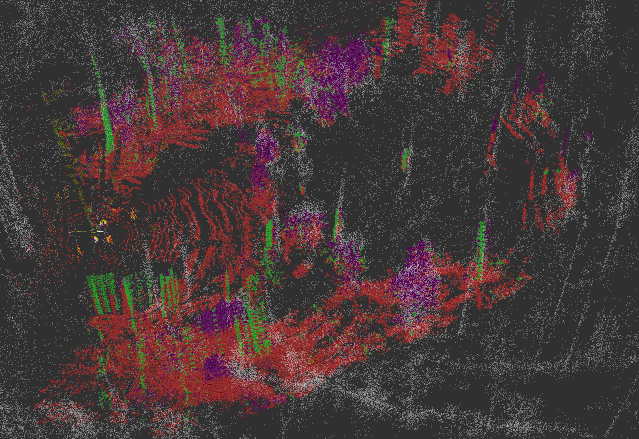
\includegraphics[width=0.8\textwidth]{figs/results/semantic_mapping/semantic_cloud_first_approach.png}
    \caption{Semantic mapping results on the Oporto test site. Fuel is red, trunks are green, canopy is purple, and background is black. White points are unlabeled. A video showing the same scene can be seen at \href{https://drive.google.com/file/d/1zulFi7uEZI8R40l-mDwUEBklhR7Kk2_1/view?usp=sharing}{this link}}
    \label{fig:results:semantic_mapping_original}
\end{figure}

The first experiment is conducted on the \textit{Oporto} dataset, which is collected in a clearing in Portugal with the custom payload at an orientation of 30 degrees from horizontal. For semantic segmentation, we use the model trained on \textit{Sete Fontes}. For localization, we use the vision-LiDAR SLAM system from \cite{RussellUnmannedMitigation}.
The results are shown in Figure \ref{fig:results:semantic_mapping_original}. This shows that the system was able to determine that there was significant fuel at ground level and correctly identify the tree trunks in the environment. The latter is important because trunks could be used as a localization aid in a similar way to SLOAM \cite{Chen2020SLOAM:Inventory}. One issue that we observed was that multiple scans were not perfectly registered with each other. This is in contrast to the final point cloud derived from SLAM, where fine details are captured precisely. Our hypothesis is that because the SLAM system uses a pose-graph \cite{Dellaert2017FactorPerception} formulation, information from loop closures can be used to update the historical pose to make it more accurate. However, the semantic mapping system only uses the most recent SLAM pose estimate, which is likely to be less accurate than the final optimized version.


A limitation of the first experiment was our lack of ground truth data to compare against.
In our second experiment on the \textit{Gascola} dataset, we still did not have field reference data but tried to approximate this as accurately as possible.
We chose to label an orthomosaic derived from a 3D model by hand. We used QGis \cite{QGIS_software}, an open-source software for interacting with geospatial data. We labeled three coarse classes, fuel, canopy, and background, which included bare-earth and other non-flammable material. Trunks were not included because they could almost never be observed in the top-down view from the orthomosaic. This manual process took approximately eight hours to complete and is visualized on the left side of Figure \ref{fig:results:semantic_map_UFO}.

\begin{figure}[H]
    \centering
    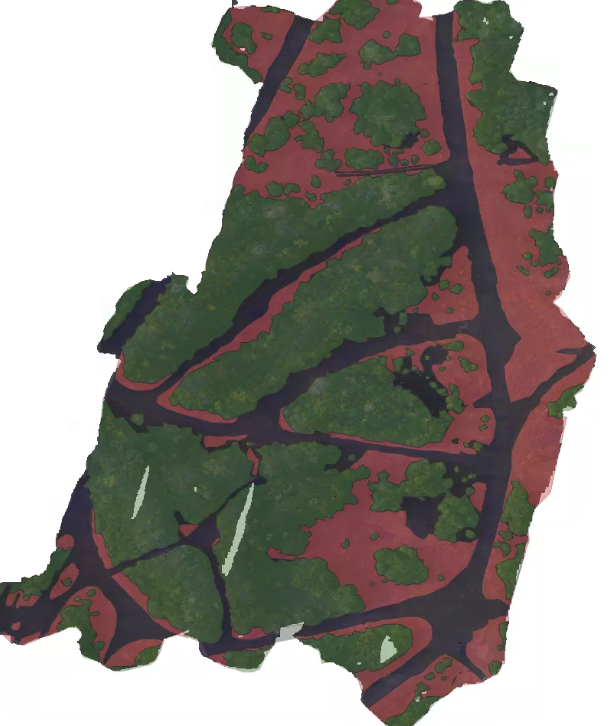
\includegraphics[width=0.40\textwidth, angle=15]{figs/results/semantic_mapping/labeled_orthomoasaic.png}
    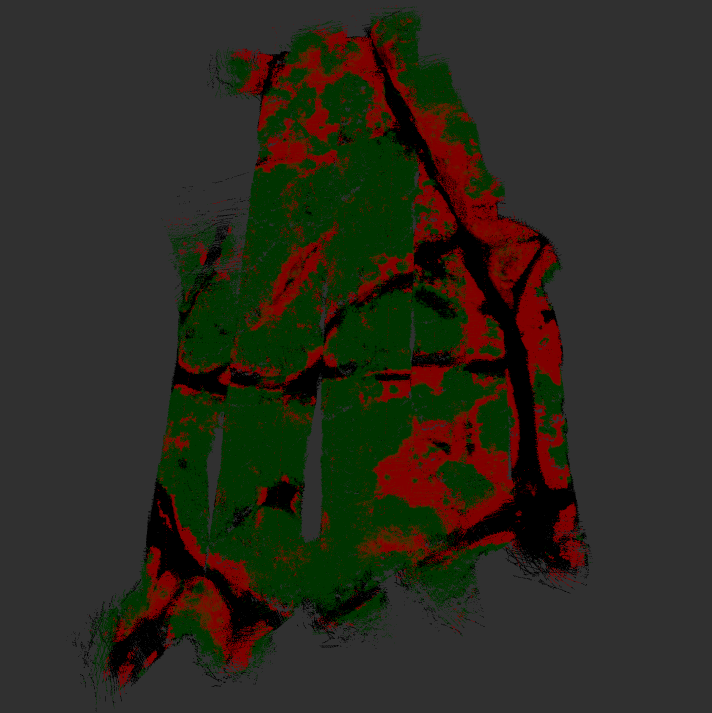
\includegraphics[width=0.45\textwidth]{figs/results/semantic_mapping/segnext_gc5_ufomap.png}
    \caption{Manually-labeled result on the left, results from UFO-Map on the right provided by M. Duda Andrada, using the SegNext \cite{Guo2022SegNeXt:Segmentation} model trained on Gascola Data.}
    \label{fig:results:semantic_map_UFO}
\end{figure}

In this experiment, we used the SegNext model trained on the manually-labeled dataset from the flight that was not used for mapping. We used the localization LIO-SAM \cite{Shan2020LIO-SAM:Mapping} and provided by Franciso Yandun to estimate the pose. In this case, we used UFOMap \cite{Duberg2020UFOMap:Unknown} instead of octomap to aggregate the observations, because of the improved performance. This change was implemented by Duda Andrada and she conducted the experiments reported here. The results of this are shown in Figure \ref{fig:results:semantic_map_UFO}. The overall structure of the scene matches well and small local features are correctly identified. One major source of error is seen in the misregistration of data from adjacent drone flights. This is seen in the vertical offsets that are especially visible on the left side of the map. This may be due to latency in the processing or also because of using the un-refined pose as described previously. The quality of this result suggests that with additional work to properly register the scans, this system could be a powerful tool for vegetation mapping. 

\section{Informative Path Planning for Commodity Drones}

\begin{figure}
    \centering
    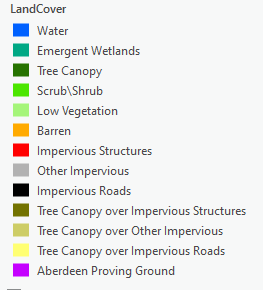
\includegraphics[width=0.3\textwidth]{figs/results/ipp/chesapeake/chesapeake_classes.png}\\
    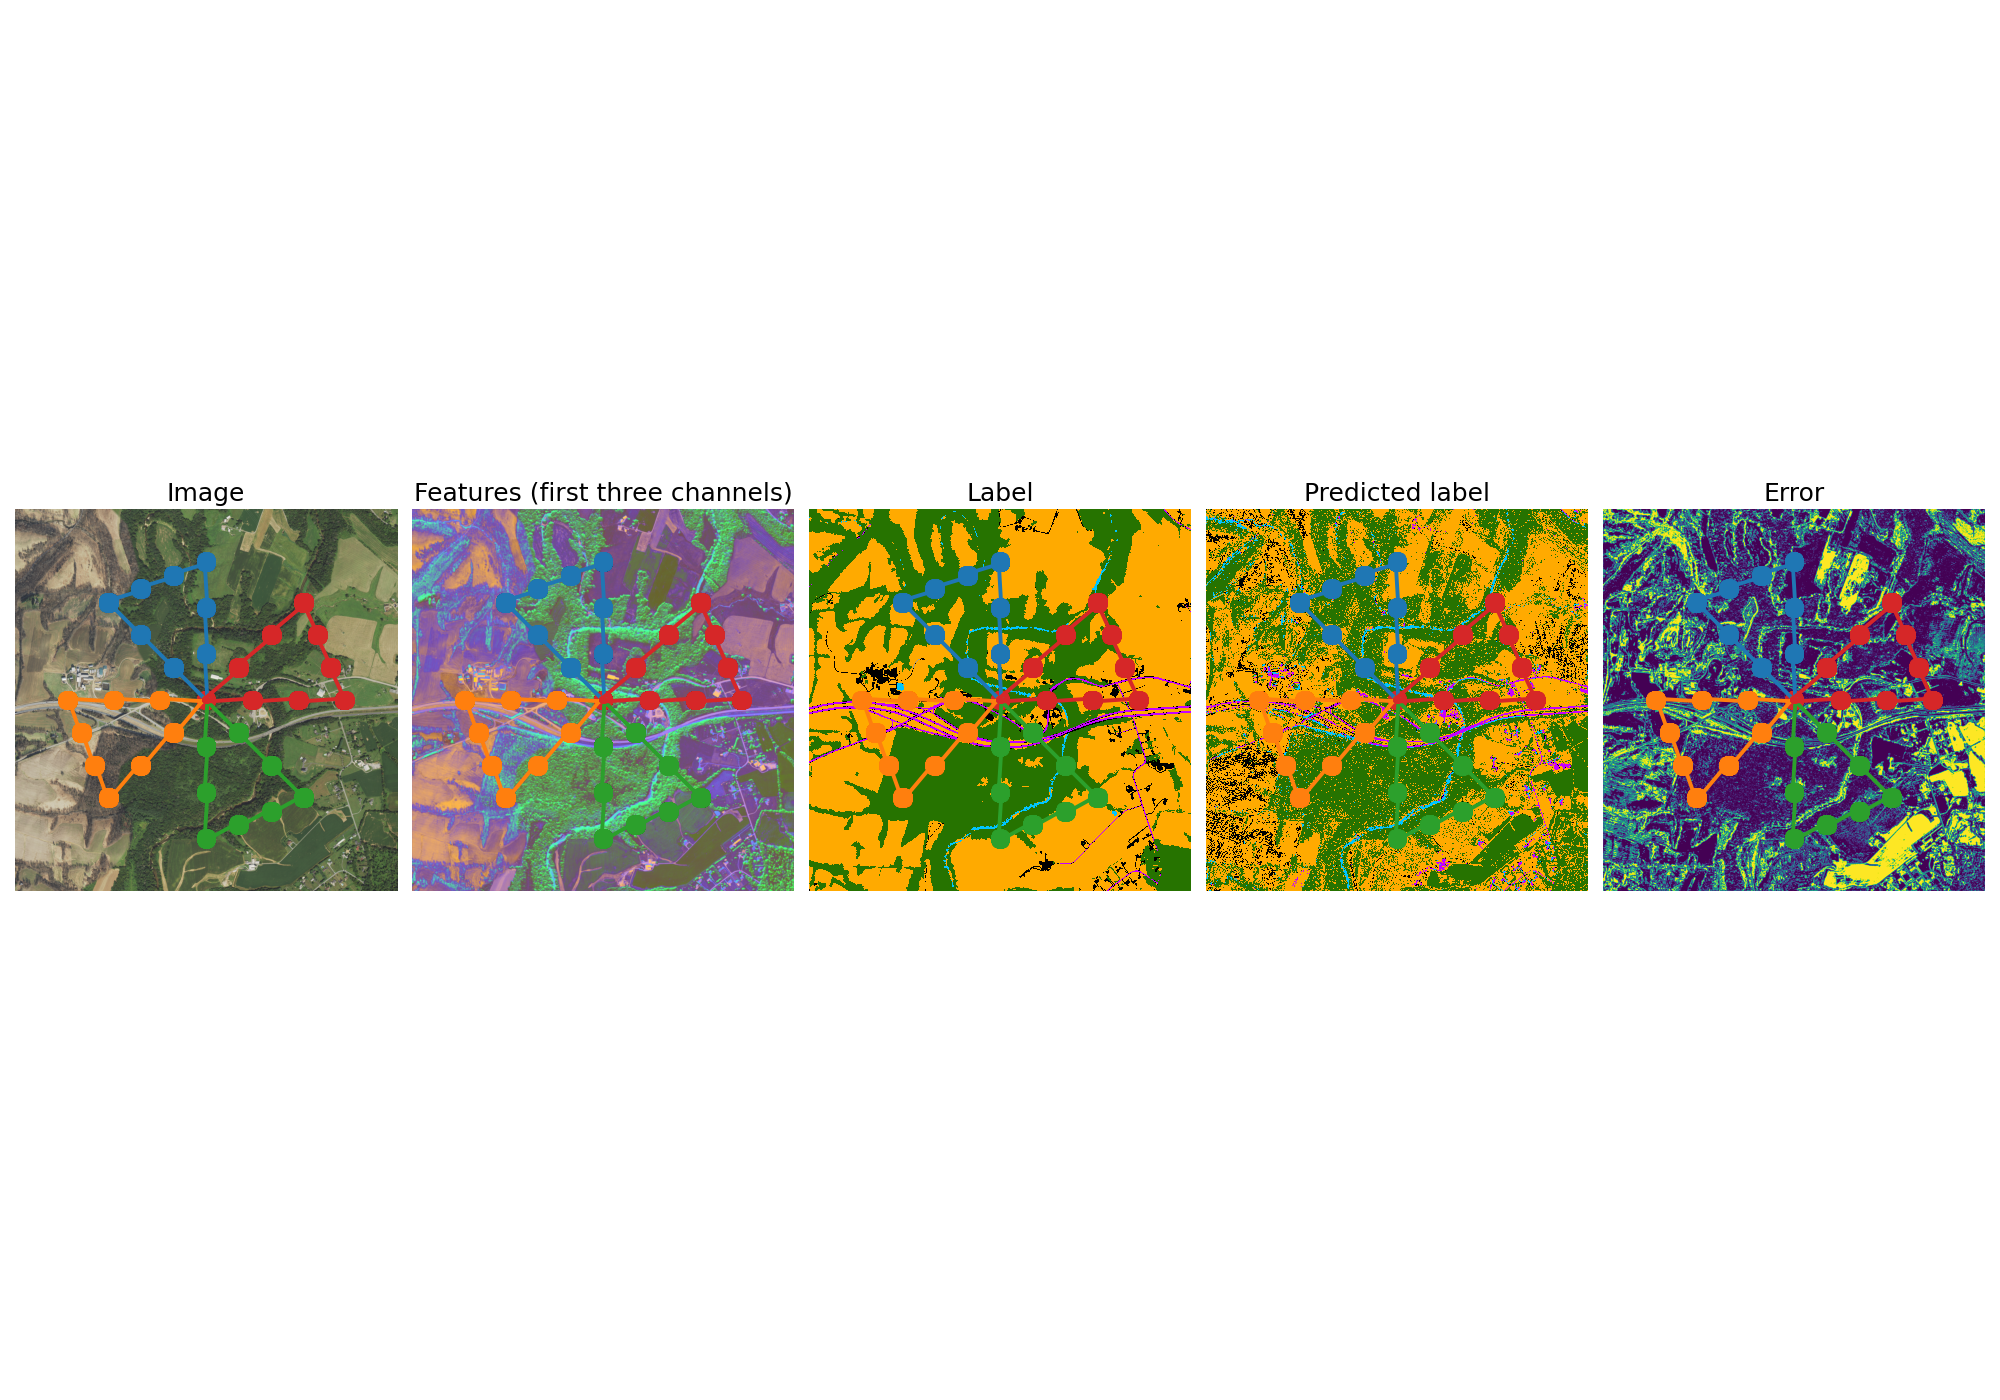
\includegraphics[width=\textwidth, trim={0 16cm 0 16cm}, clip]{figs/results/ipp/4000/paired_qual/coverage.png}
    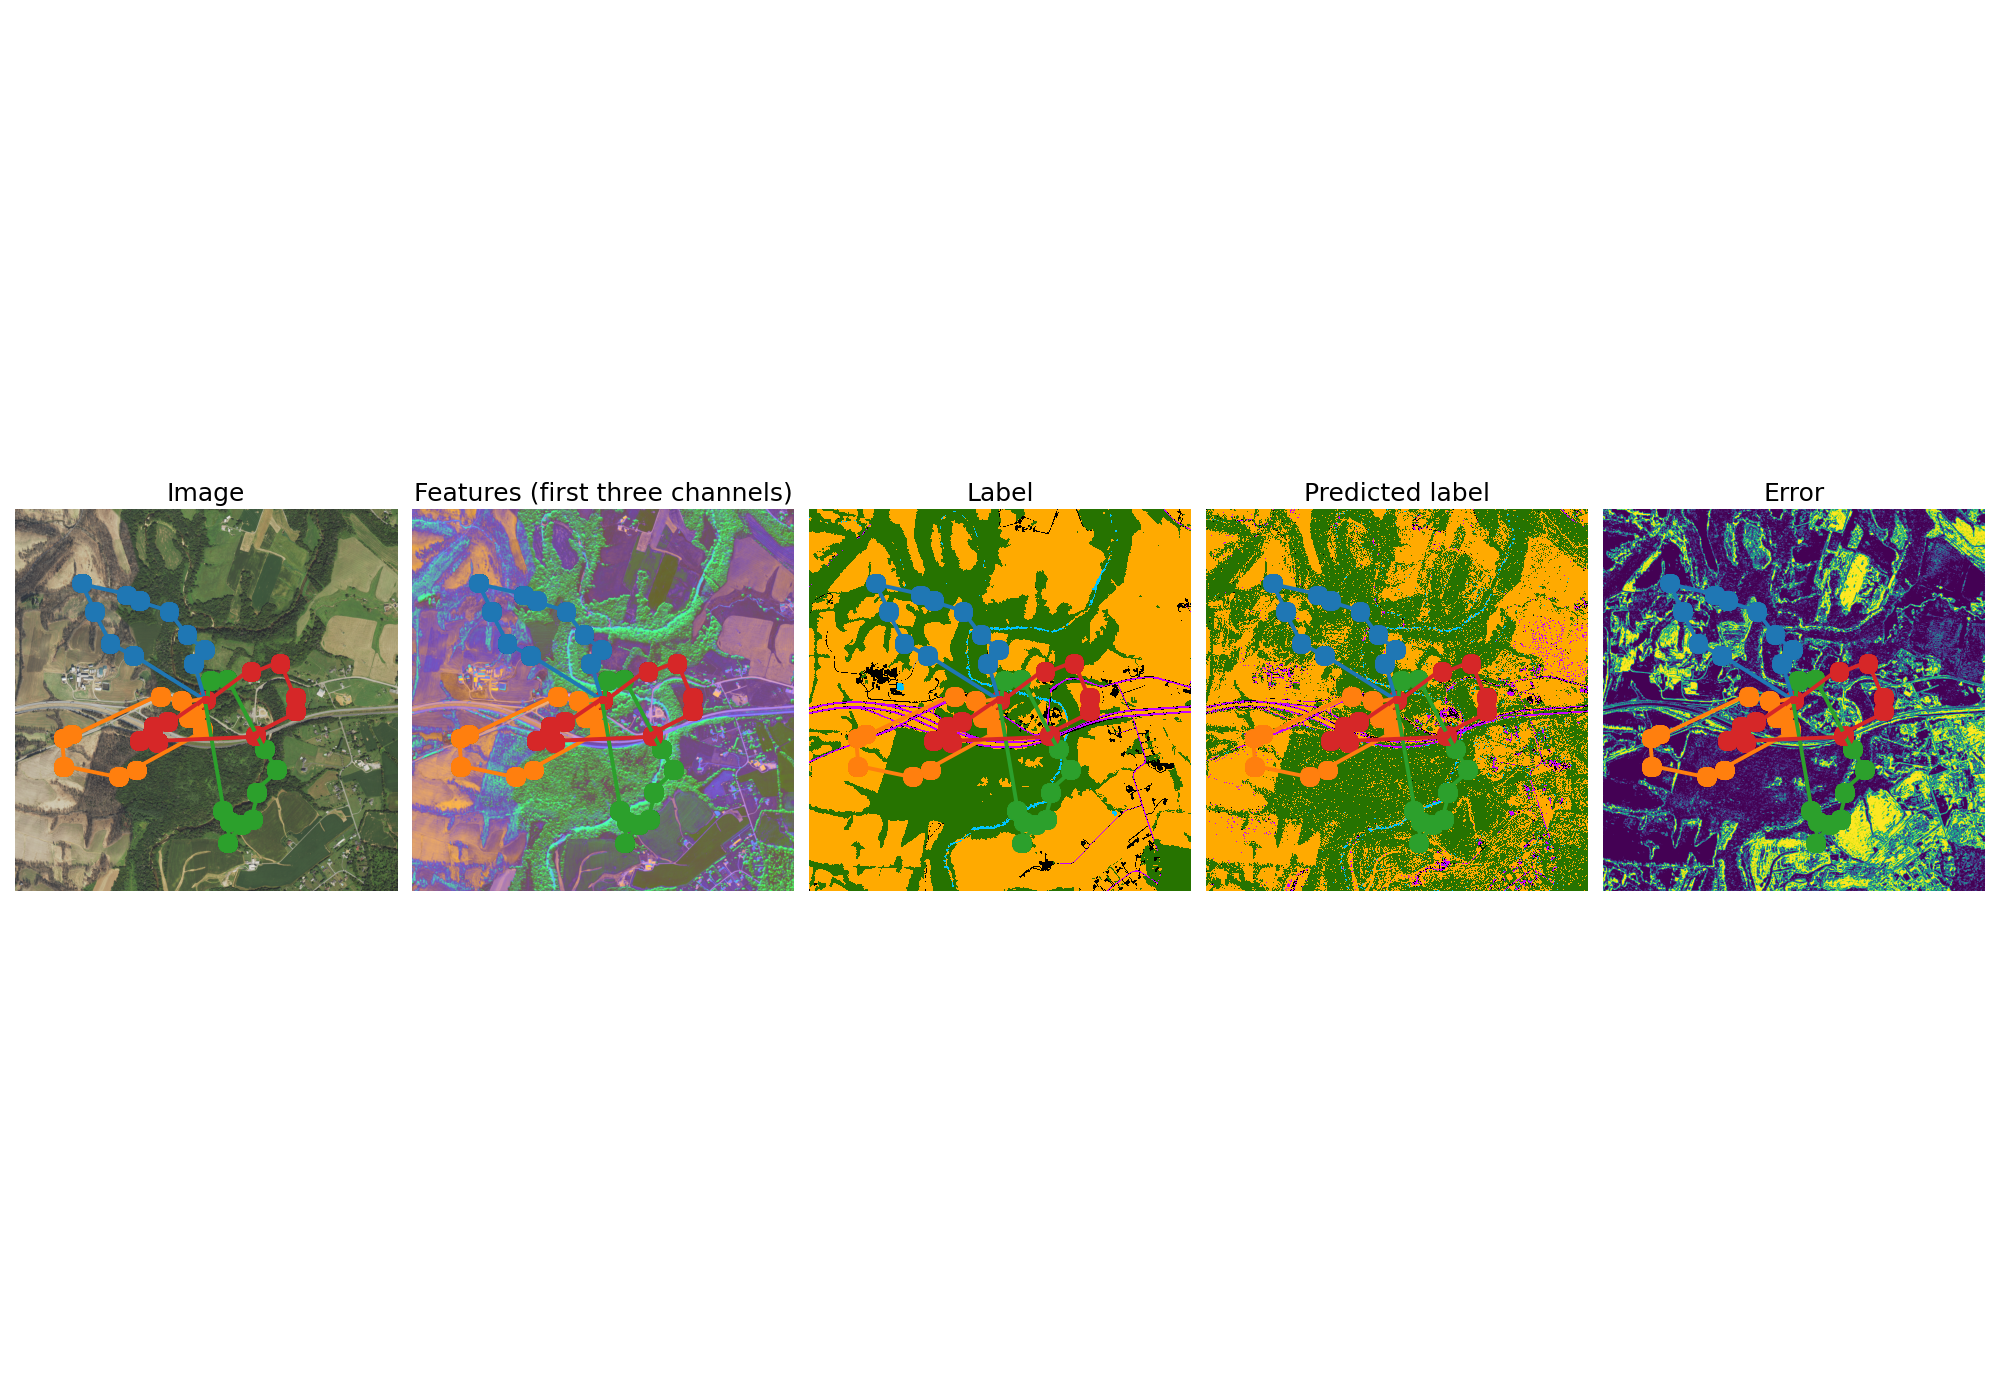
\includegraphics[width=\textwidth, trim={0 16cm 0 16cm}, clip]{figs/results/ipp/4000/paired_qual/raptors.png}
    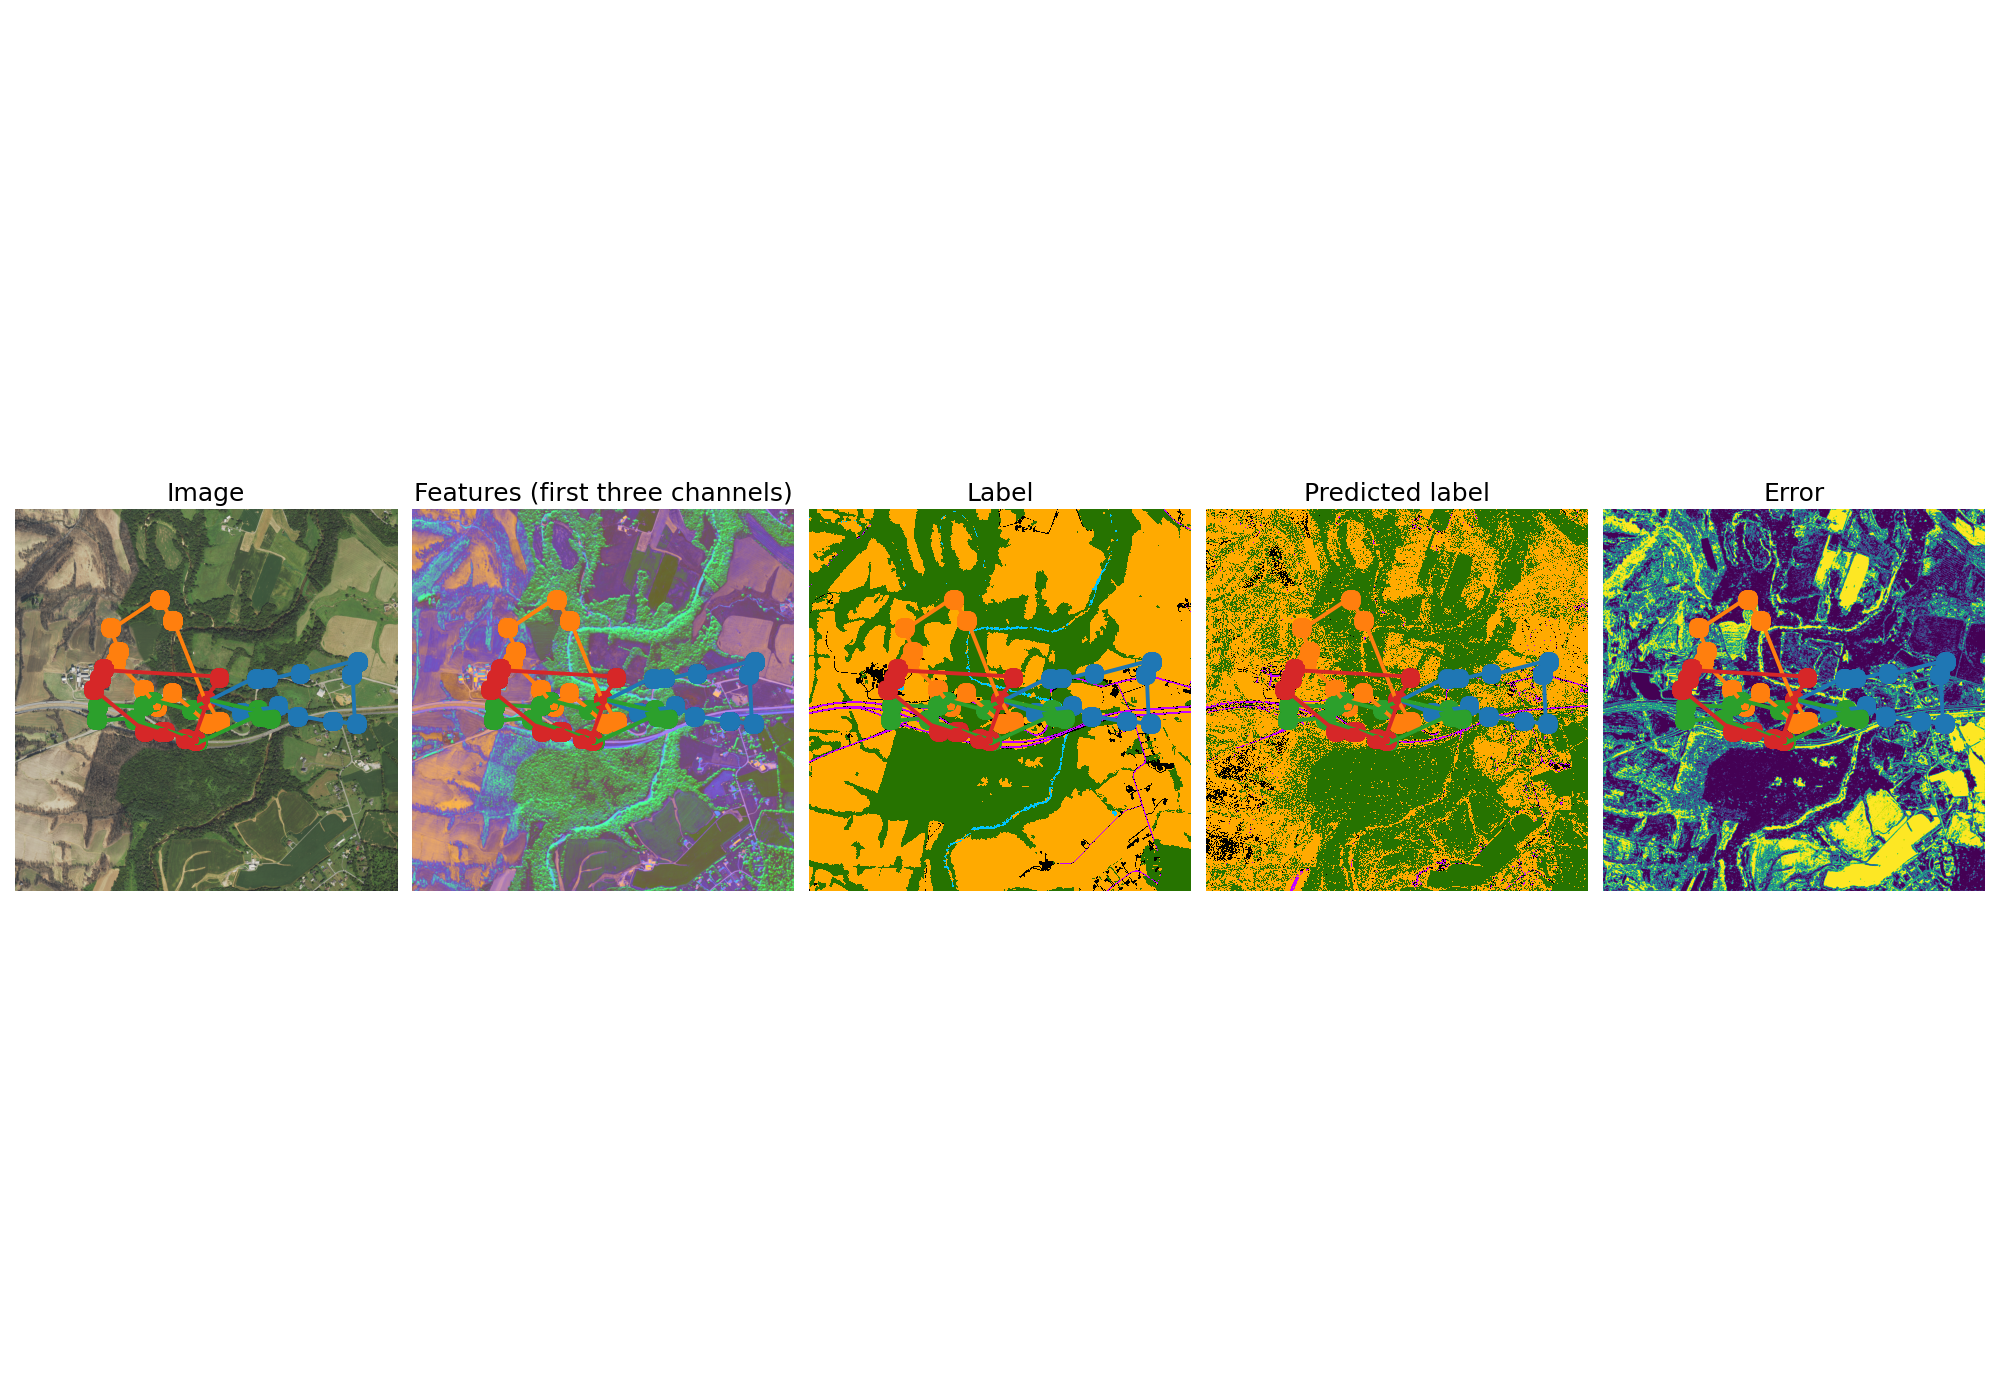
\includegraphics[width=\textwidth, trim={0 16cm 0 16cm}, clip]{figs/results/ipp/4000/paired_qual/raptors_rare.png}
    \caption{Visualizations of the coverage, RAPTORS, and RAPTORS\_rare planners from top to bottom. Each color represents an individual flight and they were executed in the following order: blue, orange, green, then red.}
    \label{fig:results:ipp_pairqual}
\end{figure}
The goal of this experiment is to simulate a land cover mapping mission for a region that is too large for the drone to exhaustively survey. Remote sensing data is available beforehand and is used to both inform the mission and generate predictions on the regions that are not observed by the drone. In this experiment, we use NAIP data \cite{U.S.DepartmentofAgriculture2011NationalSheet} and manual land cover classification annotations from the Chesapeake Bay \cite{Claggett2014ChesapeakeProduction}. We conduct experiments on a single region near Brownsville, Delaware (38°52.66', -75°41.46') that was presented in the author's data exploration example. This region consists of a patchwork of farm fields and forests with diverse appearances. 

In these experiments, we use a simple prediction system to predict the class of unobserved pixels. It is simply a k nearest-neighbor (k=7) classifier that operates on the same PCA-compressed MOSAIKS features that are used for planning. This approach is well-suited to the extremely low number of training samples used in this setting and the standardized and uncorrelated nature of our feature space.

Before any missions have been executed, the agent can only observe the label of the pixel it is at. Then it plans a mission and executes it, observing the labels at the chosen sampling locations. These samples are used to train a prediction model which is used for evaluation and can be used to inform the plan for the next mission. 

The experiments were conducted on ten random crops drawn from the region in question. Each of the approaches is run on all of the ten regions individually. Each crop is 4000x4000 pixels, representing a square with 2.4km sides. The agent starts and ends each mission in the center and the path length was set as 4000 pixels (2.4km). This meant that the agent could go to one side of the environment and return to the start within the budget but the corners were completely unreachable. Each domain was explored using four missions where 10 samples could be collected during each one. Each sample meant the agent could observe the class of a 31x31 pixel (18 meters) square region. After each mission, the class of all pixels is predicted using the KNN classifier, and the error metrics are computed.

The quality of the predictions is evaluated on two metrics: accuracy and averaged recall. The first is the fraction of pixels in the map that were assigned the correct class label by the prediction system. The second represents the average of the per-class recalls. This metric is chosen so that rare classes are treated equally in the evaluation procedure since this is critically important when we explicitly want to find rare classes. We also report the time taken to generate the plan. Note that this does not include the time taken to generate the class predictions, since the planner is agnostic to the choice of prediction algorithm.


\begin{figure}
    \subfloat{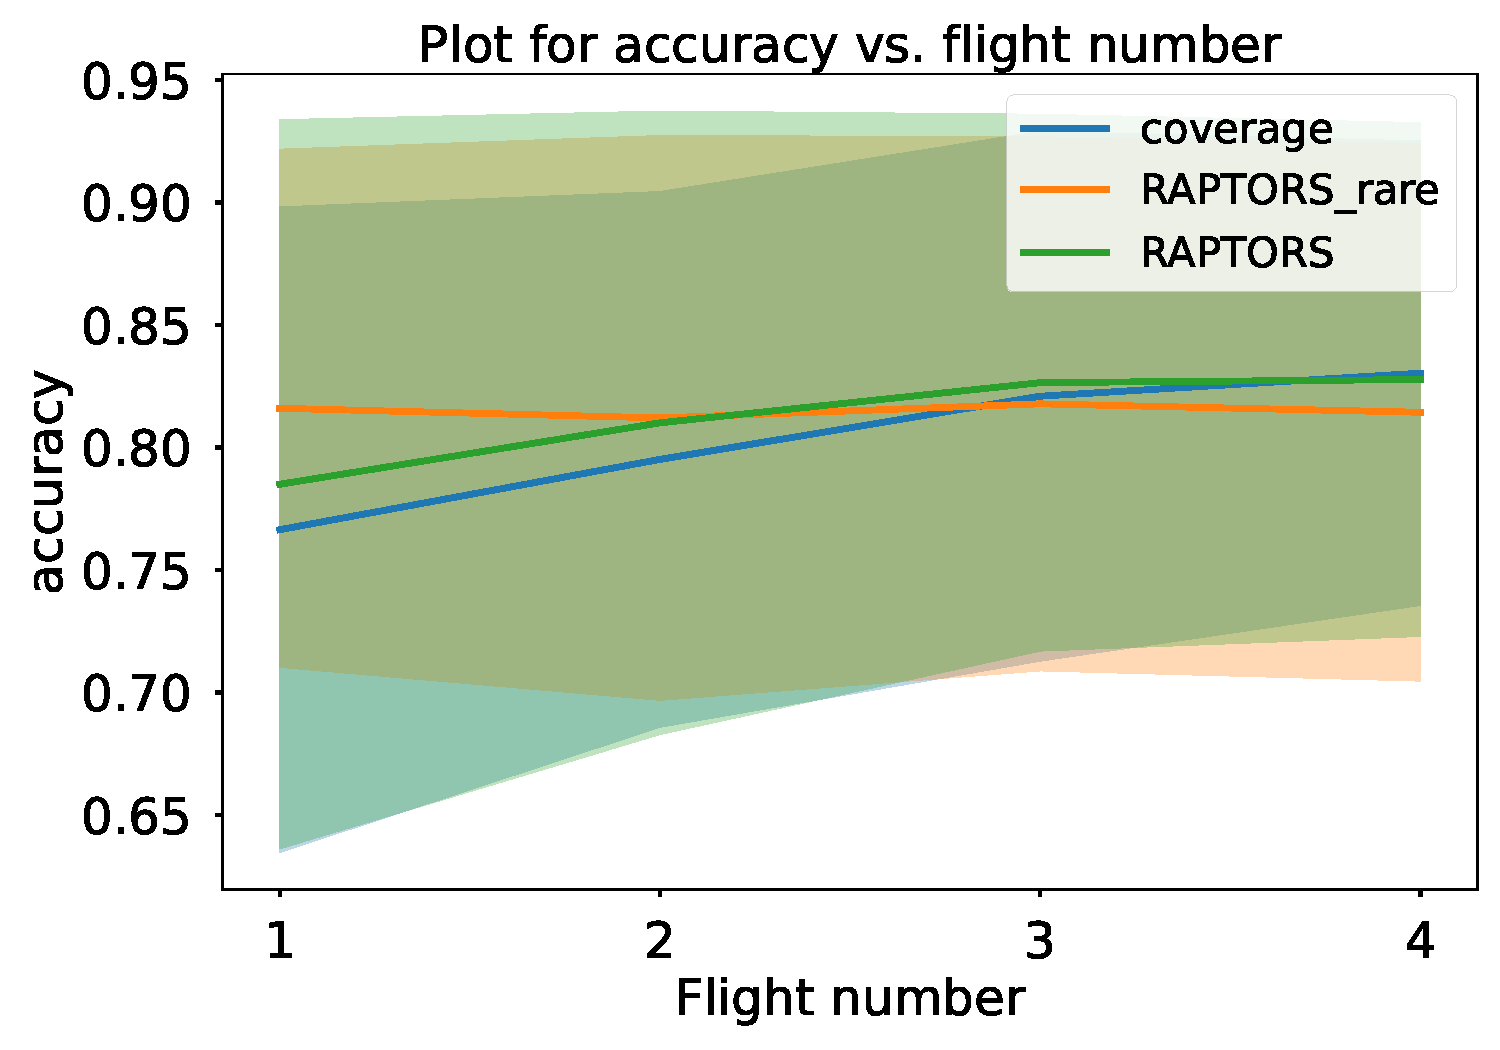
\includegraphics[width=0.5\textwidth]{figs/results/ipp/4000/accuracy.pdf}}
    \hfill
    \subfloat{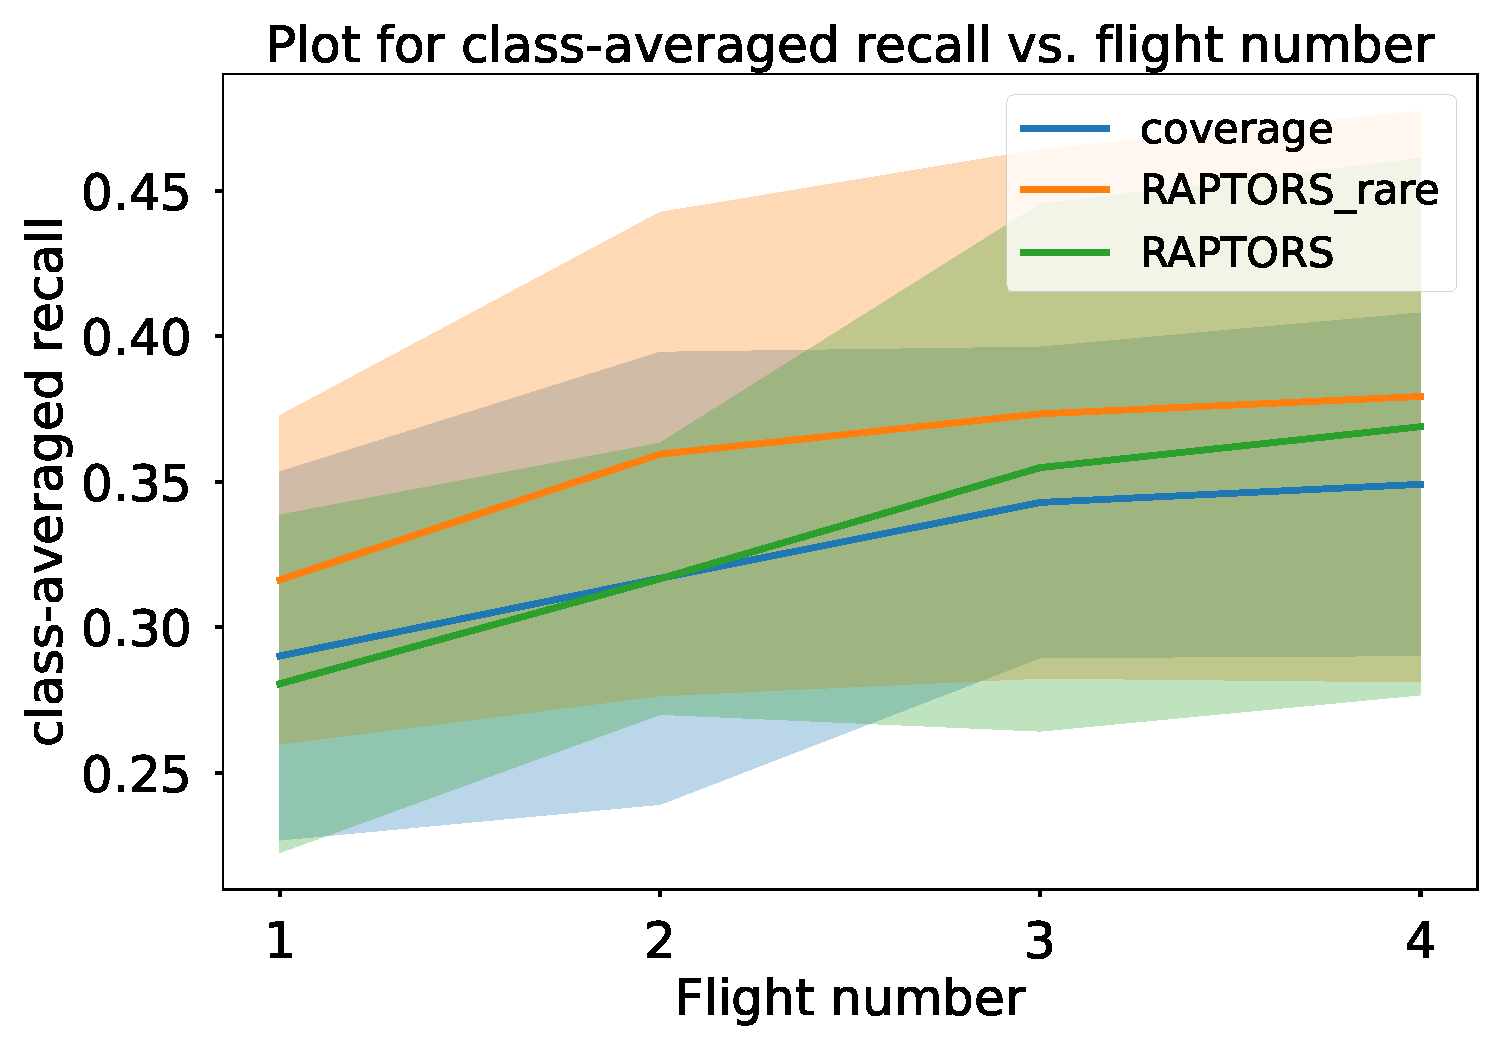
\includegraphics[width=0.5\textwidth]{figs/results/ipp/4000/class-averaged recall.pdf}}
    \hfill
    \caption{Quantitative statistics computed after each flight and averaged across 10 missions. The shaded regions represent the first standard deviation. The left result shows the accuracy and the right shows the class-averaged recall. In both cases higher is better. The proposed methods are only slightly better in terms of error on early flights and the performance converges with the coverage baseline after all flights have been completed. However, the RAPTORS variant that prioritizes rare classes achieves better recall of rare classes after any number of flights. Note that the variance of all methods is high.}
    \label{fig:results:ipp_quant}
\end{figure}

The proposed planner is compared to a hand-designed coverage approach. The path consists of a triangular pattern that begins and ends at the central location. This triangle is sized appropriately to exhaust the available path budget. The goal of this path is to cover a diverse set of locations after the four mapping missions have been completed. This planner is visualized alongside the RAPTORS methods in Figure \ref{fig:results:ipp_pairqual}. As seen there, the RAPTORS methods prioritize collecting a diverse set of samples that span the magory types of land cover. The variant that priritizes rare classes can be seen to place more samples on the road that cuts across the center of the region.

Quantitative evaluations results are presented Figure~\ref{fig:results:ipp_quant}. For all approaches, the performance improves as more samples are collected. The RAPTORS approaches have slightly better total accuracy than the coverage planner in initial flights, but the performance converges over time. This suggests that the quality of the predictions is saturating, especially for the well-represented classes. This is un-surprising because KNN is a simple prediction model. When these approaches are evaluated on class-averaged recall, which weights rare classes equallly, the RAPTORS\_rare method does better for any number of flights. This suggests that it is able to find a diverse set of initial samples and then leverage the predictions after each flight to prioritize sampling regions predicted to be rare classes. However, across all the experiments the scale of the variance is much higher than the difference between approaches. This variance partially captures the difference in difficulty between the different random sites that the approach was evaluated on. This highlights the challenge of evaluating informative path planning in a rigorous manner. The planning time for either RAPTORS variant was approximately 200 seconds per path. These experiments were executed on high-end cloud infastructure, but this shows that the approach has potential to be deployed in a realistic field scenario in the future.

%\begin{figure}
%    \centering
%    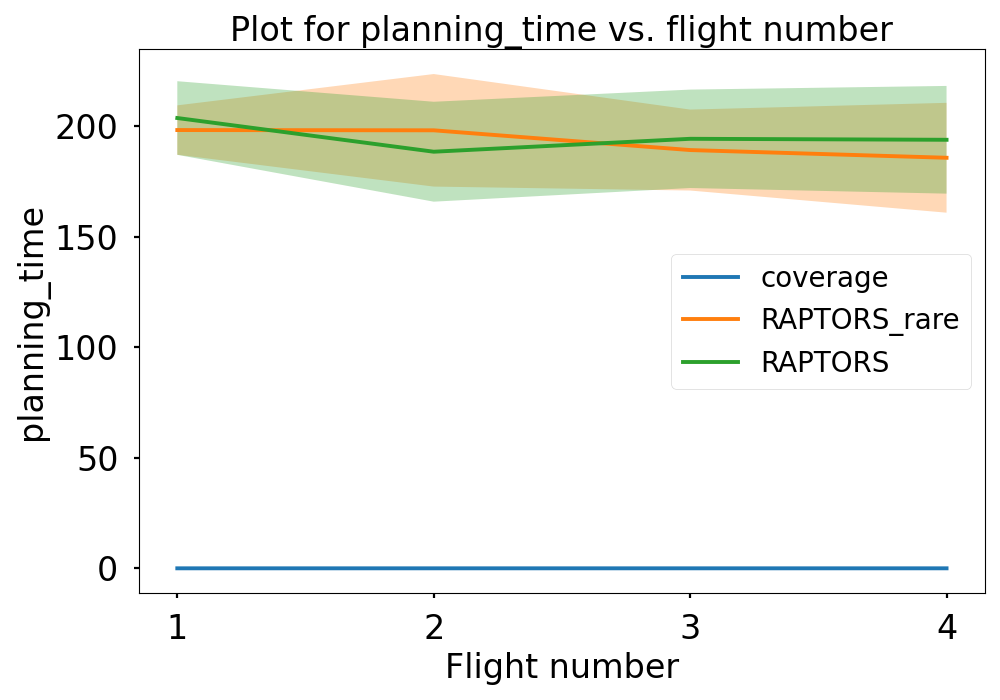
\includegraphics[width=0.6\textwidth]{figs/results/ipp/4000/planning_time.png}
%    \caption{The planning time for each flight. The RAPTORS variants take approximately 200 seconds to plan each flight, while the coverage plan can be computed instantly. }
%    \label{fig:res:ipp_timing}
%\end{figure}